%-------------------------------------------------------%
%       Snakemake-Intro for HPC Users                   %
%-------------------------------------------------------%


% this code will compile the document as handout with
% $ pdflatex -synctex=1 -interaction=nonstopmode "\def\ishandout{1} %-------------------------------------------------------%
%       Snakemake-Intro for HPC Users                   %
%-------------------------------------------------------%

\documentclass[english,xcolor=pdftex,dvipsnames]{beamer} 

% to typeset only a few slide sets, set them here during development
%\includeonly{Why_Workflows}

\usepackage{etoolbox}
%\setbeamertemplate{mini frames}[box]
\usepackage{babel}
\usepackage[utf8]{inputenc}
\usepackage[T1]{fontenc}
\usepackage{amsfonts,amsmath,amssymb}
\usepackage{textgreek}
\usepackage{wrapfig}

\usepackage[load-configurations=binary,binary-units=true]{siunitx}
\usepackage[normalem]{ulem} % for strikethrough with \sout

\usepackage{color,colortbl}
\usepackage{upquote}

\definecolor{pblue}{RGB}{45,106,148}
\definecolor{pdarkblue}{RGB}{35,71,100}
\definecolor{plightblue}{RGB}{90,159,212}
\definecolor{pyellow}{RGB}{255,212,59}
\definecolor{pdarkyellow}{RGB}{255,188,41}
\definecolor{orange}{RGB}{255,165,0}
\definecolor{plightyellow}{RGB}{255,232,115}
\definecolor{pdarkgrey}{RGB}{100,100,100}
\definecolor{pgrey}{RGB}{153,153,153}
\definecolor{plightgrey}{RGB}{233,233,233}
\definecolor{plightgrey2}{RGB}{247,247,247}
\definecolor{pnavy}{RGB}{0,0,170}
\definecolor{BrickRed}{RGB}{150,22,11}
\definecolor{BlueViolet}{RGB}{138, 43, 226}
\definecolor{PineGreen}{RGB}{0, 51, 0}
\definecolor{light-gray}{gray}{0.95}

\definecolor{UniRot}{RGB}{193,0,42}
\definecolor{UniDunkelGrau}{RGB}{99,99,99}
\definecolor{UniHellGrau}{RGB}{172,172,172}

\definecolor{UrlColor}{rgb}{0,0.08,0.45}
\definecolor{links}{rgb}{0,0,0}

\usetheme{CambridgeUS} % Pittsburgh, CambridgeUS
\usecolortheme{beaver} %wolverine | crane | beaver | seahorse
\useinnertheme{rounded} 
\useoutertheme{default}
\usefonttheme{default}
%\setbeamercovered{transparent}
\setbeamertemplate{footline}[frame number]

% remove the navigation symbols
\setbeamertemplate{navigation symbols}{}

% side margins
\setbeamersize{text margin left=0.5cm, text margin right=0.5cm}

\setbeamercolor{structure}{fg=UniRot}% to modify  immediately all palettes
\setbeamercolor{title}{fg=UniRot}
\setbeamercolor{title in head/foot}{fg=UniRot}

\setbeamercolor{block title}{bg=UniRot!20,fg=darkred}
\setbeamercolor{block body}{fg=black, bg=plightgrey2}

% \setbeamercolor{block title}{fg=white,bg=orange}
\setbeamercolor{block title alerted}{fg=white,bg=UniRot}
\setbeamercolor{block title example}{fg=white,bg=PineGreen!80}


% enables two line cols in tabular envs
\newcommand{\specialcell}[2][c]{%
  \begin{tabular}[#1]{@{}c@{}}#2\end{tabular}}
\usepackage{subfig}
\usepackage{tikz}
\usetikzlibrary{arrows,shapes,backgrounds,positioning,shadows,decorations,trees,decorations.pathreplacing}
\usepackage{tkz-graph}

\usepackage{smartdiagram}


\addtobeamertemplate{footline}{}{%
\begin{tikzpicture}[remember picture,overlay]
\node[anchor=south west,yshift=2pt] at (current page.south west) {\includegraphics[height=0.8cm]{../images/logos/zdv_logo.png}};
\end{tikzpicture}}

\usepackage[tikz]{bclogo}
\newenvironment{task}[1][Task]{\bclogo[arrondi=0.1,logo=\bcoutil]{#1}}{\endbclogo}
\newenvironment{docs}[1][Documentation]{\bclogo[arrondi=0.1,logo=\bcplume]{#1}}{\endbclogo}
\newenvironment{hint}[1][Hint]{\bclogo[arrondi=0.1,logo=\bcinfo]{#1}}{\endbclogo}
\newenvironment{warning}[1][Warning]{\bclogo[arrondi=0.1,logo=\bcattention]{#1}}{\endbclogo}
% ``d/Definition'' is already defined ;-)
\newenvironment{explanation}[1][Definition]{\bclogo[arrondi=0.1,logo=\bcplume]{#1}}{\endbclogo}
\newenvironment{question}[1][Question]{\bclogo[arrondi=0.1,logo=\bcquestion]{#1}}{\endbclogo}


%%%%%%%%%%%%%%%%%
%% PLEASE NOTE %%
%%%%%%%%%%%%%%%%%
% frames containing ``Hand Out'' or ``Interlude'' should be started:

% \setcounter{preframe_handson}{\value{handson}}
% \begin{frame}[fragile]
%   \setcounter{handson}{\value{preframe_handson}}
%   \frametitle{\HandsOn{Using \texttt{find}}}

% or

% \setcounter{preframe_interlude}{\value{interlude}}
% \begin{frame}[fragile]
%   \setcounter{interlude}{\value{preframe_interlude}}
%   \frametitle{Interlude -- Parameter Extension}

% respectively.

\newcounter{handson}
\setcounter{handson}{1}
\newcounter{preframe_handson}
\setcounter{preframe_handson}{1}
\newcommand{\HandsOn}[1]{Hands On \Roman{handson} -- #1 \addtocounter{handson}{1}}
%\newcommand{\HandsOn}[1]{Hands On -- #1}

%TODO: Merge ``HandsOn'' && ``Excercise''
\newcounter{exercise}
\setcounter{exercise}{1}
% \newcommand{\Exercise}{\theexercise . Excercise \addtocounter{exercise}{1}}

% Bugfix of the Exercise command: avoid the annoying counter
\newcommand{\Exercise}{\theexercise . Excercise \addtocounter{exercise}{1}}

\newcounter{interlude}
\setcounter{interlude}{1}
\newcounter{preframe_interlude}
\setcounter{preframe_interlude}{1}

%\newcommand{\Interlude}[1]{Interlude \Roman{interlude} -- #1 \addtocounter{interlude}{1}}

% Bugfix of the Interlude command: avoid the annoying counter!
\newcommand{\Interlude}[1]{Interlude -- #1}

\usepackage{marvosym}
\usepackage{multicol}

\usepackage{hhline}

\usepackage{times}

% will decrease the font size for one frame
\newcommand\Fontvi{\fontsize{6}{7.2}\selectfont}
% 
\usepackage{dirtree,float} % for directory tree listings
\usepackage[nodisplayskipstretch]{setspace}


\usepackage{verbatim}
\usepackage{listings}

\newcommand{\altverb}[2][{}]{\colorbox{plightgrey}{\lstinline[language={#1}]{#2}}}


\lstloadlanguages{Python,bash,C++}
\lstset{showspaces=false,
basicstyle=\small,
showstringspaces=false}

\lstdefinestyle{tree}{
    literate=
    {├}{{smash{raisebox{-1ex}{rule{1pt}{baselineskip}}}raisebox{0.5ex}{rule{1ex}{1pt}}}}1 
    {─}{{raisebox{0.5ex}{rule{1.5ex}{1pt}}}}1 
    {└}{{smash{raisebox{0.5ex}{rule{1pt}{dimexprbaselineskip-1.5ex}}}raisebox{0.5ex}{rule{1ex}{1pt}}}}1 
  }

%default python listings:
\lstdefinestyle{Python}
{
  language=Python,
  basicstyle=\small,
  showstringspaces=false,
  stepnumber=5,
  numberstyle=\tiny,
  numbersep=5pt,
  showspaces=false,
  frame=single,
  framerule=0.4pt,
  rulecolor=\color{pgrey},
  backgroundcolor=\color{white},
  stringstyle=\color{BrickRed},
  keywordstyle=\color{BlueViolet}\bfseries,
  commentstyle=\color{PineGreen}\bfseries,
  identifierstyle={},
  emph={[10]self}, emphstyle={[10]\color{pblue}},
  emph={[11]yield}, emphstyle={[11]\color{pblue}},
  moredelim=**[is][\bfseries\color{red}]{@}{@},
  literate={\\@}{{\makeatletter @ \makeatother}}1
}

\lstdefinestyle{R}
{
  language=R,
  basicstyle=\small,
  showstringspaces=false,
  stepnumber=5,
  numberstyle=\tiny,
  numbersep=5pt,
  showspaces=false,
  frame=single,
  framerule=0.4pt,
  rulecolor=\color{pgrey},
  backgroundcolor=\color{white},
  stringstyle=\color{BrickRed},
  keywordstyle=\color{BlueViolet}\bfseries,
  commentstyle=\color{PineGreen}\bfseries,
  identifierstyle={},
  emph={[10]self}, emphstyle={[10]\color{pblue}},
  emph={[11]yield}, emphstyle={[11]\color{pblue}},
}

%default python listings:
\lstdefinestyle{C++}
{
  language=C++,
  basicstyle=\small,
  showstringspaces=false,
  stepnumber=5,
  numberstyle=\tiny,
  numbersep=5pt,
  showspaces=false,
  frame=single,
  framerule=0.4pt,
  rulecolor=\color{pgrey},
  backgroundcolor=\color{white},
  stringstyle=\color{BrickRed},
  keywordstyle=\color{BlueViolet}\bfseries,
  commentstyle=\color{PineGreen}\bfseries,
  identifierstyle={},
  emph={[10]self}, emphstyle={[10]\color{pblue}},
  emph={[11]yield}, emphstyle={[11]\color{pblue}},
}

\newcommand{\CC}{C\nolinebreak\hspace{-.05em}\raisebox{1ex}{\tiny\bf +}\nolinebreak\hspace{-.10em}\raisebox{1ex}{\tiny\bf +}}

%default shell listings:
\lstdefinestyle{Shell}
{
  language=Bash,
  basicstyle=\ttfamily\small,
  showstringspaces=false,
  frame=single,
  framerule=0.4pt,
  rulecolor=\color{pgrey},
  backgroundcolor=\color{plightgrey2},
  stringstyle=\color{BrickRed},
  keywordstyle=\color{BlueViolet},
  commentstyle=\color{PineGreen}\bfseries,
  identifierstyle=\color{black},
  emph={[10]\$,>>>}, emphstyle={[10]\color{pblue}},
  moredelim=**[is][\bfseries\color{red}]{@}{@},
  literate={\\@}{{\makeatletter @ \makeatother}}1
}

%default plain listings (e.g. for config files):https://www.google.com/search?client=firefox-b-e&q=conrad
\lstdefinestyle{Plain}
{ 
  stepnumber=5,
  numberstyle=\tiny,
  numbersep=5pt,
  language=Bash,
  basicstyle=\ttfamily\small,
  showstringspaces=false,
  frame=single,
  framerule=0.4pt,
  rulecolor=\color{pgrey},
  backgroundcolor=\color{plightgrey2},
  stringstyle=\color{black},
  keywordstyle=\color{black},
  commentstyle=\color{blue}\bfseries,
  identifierstyle=\color{black},
  breaklines=true,
  emph={[10]\$,>>>}, emphstyle={[10]\color{pblue}}
}

\lstdefinelanguage{XML}
{
  frame=single,
  framerule=0.4pt,
  rulecolor=\color{pgrey},
  backgroundcolor=\color{plightgrey2},
  stringstyle=\color{black},
  keywordstyle=\color{black},
  commentstyle=\color{blue}\bfseries,
  identifierstyle=\color{black},
  emph={[10]\$,>>>}, emphstyle={[10]\color{pblue}}
  morestring=[b]",
  morestring=[s]{>}{<},
  morecomment=[s]{<?}{?>},
  morekeywords={xmlns,version,type}% list your attributes here
}

\newcommand{\bibtex}{\textsc{Bib}\TeX}

%%% https://tex.stackexchange.com/questions/99316/symbol-for-external-links
\newcommand{\LinkSymbol}{%
  \tikz[x=1.2ex, y=1.2ex, baseline=-0.05ex]{% 
    \begin{scope}[x=1ex, y=1ex]
      \clip (-0.1,-0.1) 
      --++ (-0, 1.2) 
      --++ (0.6, 0) 
      --++ (0, -0.6) 
      --++ (0.6, 0) 
      --++ (0, -1);
      \path[draw, 
      line width = 0.5, 
      rounded corners=0.5] 
      (0,0) rectangle (1,1);
    \end{scope}
    \path[draw, line width = 0.5] (0.5, 0.5) 
    -- (1, 1);
    \path[draw, line width = 0.5] (0.6, 1) 
    -- (1, 1) -- (1, 0.6);
  }
}
\newcommand{\lhref}[2]{\href{#1}{#2\,\LinkSymbol}}

%%%% shortcuts for uniform appearance of common strings %%%%
\newcommand{\slurm}{\textsc{slurm}~}
\makeatletter
\newcommand{\rmnum}[1]{\romannumeral #1}
\newcommand{\Rmnum}[1]{\expandafter\@slowromancap\romannumeral #1@}
\makeatother

% this package provides the option to read parameters from a configuration file
\usepackage{readarray}

\readdef{config/config.dat}{\data}
\readarray\data\MyDat[-,3]
\newcommand\configparam[1]{\csname DATA#1\endcsname}
%\MyDatROWS{} rows of data read.

\newcounter{datacount}
\setcounter{datacount}{0}%
\whiledo{\value{datacount} < \MyDatROWS}{%
	\stepcounter{datacount}%
	\expandafter\xdef\csname DATA\MyDat[\arabic{datacount},1]\endcsname{%
		\MyDat[\arabic{datacount},3]}%
}



%\newcommand{\pathtoexercise}[1]{\path{/lustre/project/m2_jgu-ngstraing/workflows/#1}}
%\newcommand{\pathtoexercise}[1]{\path{ \DTLfetch{data}{thekey}{#1}{thevalue}   }}
%\newcommand{\pathtoclozure}[1]{\path{/lustre/project/hpckurs/bash-course/cloze/#1}}
%\newcommand{\pathtosolution}[1]{\path{/lustre/project/hpckurs/bash-course/solutions/#1}}

\setcounter{tocdepth}{1}

% this allows turning of footlines for particular slides
\setbeamertemplate{footline}[frame number]
% to use it, perform:

% \begin{frame}
% normal frame
% \end{frame}
% 
% \begingroup
% \setbeamertemplate{footline}{}
% \begin{frame}
% without footline
% \end{frame}
% \endgroup

%--------------------%
% Meta-Info 
%--------------------%



\title[Introduction to Workflow Programming]{An Introduction to HPC-conformant Scientific Workflows} 
%TODO: What should the subtitle be like? Should there be an Edition? How to keep track?
\subtitle{Workflow Course - Edition 3} 
\author[Snakemake Teaching Alliance]{The "Snakemake Teaching Alliance"}
% TODO: How do we insert a date, which is up to date? Should we insert one, here?
\date{September 2023}

\hypersetup{colorlinks,linkcolor=,urlcolor=links}

\graphicspath{{../images/}{../logos}}


% Passe captions an
\setbeamertemplate{caption}{\insertcaption}
% \setbeamerfont{caption}{size=\scriptsize}
\setlength\abovecaptionskip{-2.5pt}
\setlength\belowcaptionskip{0pt}



% For every picture that defines or uses external nodes, you'll have to
% apply the 'remember picture' style. To avoid some typing, we'll apply
% the style to all pictures.
\tikzstyle{every picture}+=[remember picture]
\tikzstyle{na} = [baseline=-.5ex]


%%%%%%%%%%%%%%%%%%%%%%%%%%%%%%%%%%%%%%%%%%%%%%%%%%%%%%%%%%%%%%%%%%%%%%%%%%%%%%%%
%%%%%%%%%%%%%%%%%%%%%%%%%%%%%%%%%%%%%%%%%%%%%%%%%%%%%%%%%%%%%%%%%%%%%%%%%%%%%%%%
\begin{document}
%%%%%%%%%%%%%%%%%%%%%%%%%%%%%%%%%%%%%%%%%%%%%%%%%%%%%%%%%%%%%%%%%%%%%%%%%%%%%%%%
%%%%%%%%%%%%%%%%%%%%%%%%%%%%%%%%%%%%%%%%%%%%%%%%%%%%%%%%%%%%%%%%%%%%%%%%%%%%%%%%

%%%%%%%%%%%%%%%%%%%%%%%%%%%%%%%%%%%%%%%%%%%%%%%%%%%%%%%%%%%%%%%%%%%%%%%%%%%%%%%% 
\begin{frame}[plain] % plain erzeugt Titelseite ohne Kopf- und Fußzeile
  \titlepage
\end{frame}

%%%%%%%%%%%%%%%%%%%%%%%%%%%%%%%%%%%%%%%%%%%%%%%%%%%%%%%%%%%%%%%%%%%%%%%%%%%%%%%%
%%%%%%%%%%%%%%%%%%%%%%%%%%%%%%%%%%%%%%%%%%%%%%%%%%%%%%%%%%%%%%%%%%%%%%%%%%%%%%%%
\section{Contributors}

%%%%%%%%%%%%%%%%%%%%%%%%%%%%%%%%%%%%%%%%%%%%%%%%%%%%%%%%%%%%%%%%%%%%%%%%%%%%%%%%
\begin{frame}
  \frametitle{Honour where Honour is due}
  \begin{columns}
  	\begin{column}{.5\textwidth}
  	   \begin{itemize}
  	   	\item Johannes Köster \includegraphics[height=\baselineskip]{logos/signet_ude_rgb}
  	   	\item Lukas Hellmann \includegraphics[height=\baselineskip]{logos/logo_schriftzug.jpg}
  	   	\item Christian Meesters \includegraphics[height=\baselineskip]{logos/logo_schriftzug.jpg}
  	   	\item Malte Petersen \includegraphics[height=\baselineskip]{logos/UNI_Bonn_Logo_Standard+HPCA.pdf}
  	   	\item Fabian Brand \includegraphics[height=\baselineskip]{logos/UNI_Bonn_Logo_Standard+HPCA.pdf}
  	   	\item Florian Boecker \includegraphics[height=\baselineskip]{logos/UNI_Bonn_Logo_Standard_RZ.pdf}
  	   \end{itemize}	
  	\end{column}
    \begin{column}{.5\textwidth}
    	\begin{itemize}
    		\item See how to contribute \lhref{https://github.com/cmeesters/snakemake-hpc-teaching-material}{on our repository.}
    	\end{itemize}	
    \end{column}
  \end{columns}
		
\end{frame}



%%%%%%%%%%%%%%%%%%%%%%%%%%%%%%%%%%%%%%%%%%%%%%%%%%%%%%%%%%%%%%%%%%%%%%%%%%%%%%%%
\section{Why Workflows}

%%%%%%%%%%%%%%%%%%%%%%%%%%%%%%%%%%%%%%%%%%%%%%%%%%%%%%%%%%%%%%%%%%%%%%%%%%%%%%%%
\begin{frame}
    \frametitle{Outline}
    \begin{columns}[t]
        \begin{column}{.5\textwidth}
            \tableofcontents[sections={1-9},currentsection]
        \end{column}
        \begin{column}{.5\textwidth}
            \tableofcontents[sections={10-18},currentsection]
        \end{column}
    \end{columns}
\end{frame}

%%%%%%%%%%%%%%%%%%%%%%%%%%%%%%%%%%%%%%%%%%%%%%%%%%%%%%%%%%%%%%%%%%%%%%%%%%%%%%%%
\begin{frame}
  \frametitle{What is this about?}
   \begin{question}[Questions]
   	 \begin{itemize}
        \item I can code everything! Can I?
        \item What is the benefit of a workflow system?
        \item What distinguishes a workflow system from a ``pipeline''?
     \end{itemize}
   \end{question}
   \docs[Objectives]{\begin{enumerate}
                      \item Introducing workflow engines (particularly \texttt{Snakemake})!
                     \end{enumerate}}
\end{frame}  

%%%%%%%%%%%%%%%%%%%%%%%%%%%%%%%%%%%%%%%%%%%%%%%%%%%%%%%%%%%%%%%%%%%%%%%%%%%%%%%%
\begin{frame}
  \frametitle{Data Analysis}
  \begin{onlyenv}<1| handout:0>
    \begin{tikzpicture}
      \path[use as bounding box] (0.7,0) rectangle (12,8);
      \node[inner sep=0pt] (analysis_1) at (5,6)
         {\includegraphics[width=0.7\textwidth]{Snakemake/analysis_1.png}};   
      \node at (7, 3.5) %[below=-0.4cm of analysis_1, xshift=2.7cm] at (current page.center)
         {\includegraphics[width=0.45\textwidth]{Snakemake/phd_left.png}};
      \node at (6, 1) {\begin{minipage}{0.75\textwidth}\footnotesize
                        Idea from the official \lhref{https://slides.com/johanneskoester/snakemake-tutorial}{\texttt{Snakemake}} course (with permission), image from \lhref{https://phdcomics.com/comics.php}{PhD comics}.
                       \end{minipage}
      };
    \end{tikzpicture}    
  \end{onlyenv}
  
  \begin{onlyenv}<2| handout:1>
    \begin{tikzpicture}
      \path[use as bounding box] (0.7,0) rectangle (12,8);
      \node[inner sep=0pt] (analysis_full) at (5,6)
         {\includegraphics[width=0.7\textwidth]{Snakemake/analysis_full.png}};   
      \node at (7,3.5) % [below=-0.4cm of analysis_full, xshift=2.7cm]
         {\includegraphics[width=0.45\textwidth]{Snakemake/phd_full.png}};
      \node at (6, 1) {\begin{minipage}{0.75\textwidth}\footnotesize
                        Idea from the official \lhref{https://slides.com/johanneskoester/snakemake-tutorial}{\texttt{Snakemake}} course (with permission), image from \lhref{https://phdcomics.com/comics.php}{PhD comics}.
                       \end{minipage}
      };
    \end{tikzpicture}
  \end{onlyenv}
\end{frame}

%%%%%%%%%%%%%%%%%%%%%%%%%%%%%%%%%%%%%%%%%%%%%%%%%%%%%%%%%%%%%%%%%%%%%%%%%%%%%%%%
\begin{frame}
  \frametitle{Goals of Reproducibility}
  \Huge
  \begin{enumerate}
   \item Dispel Doubts
   \item Facilitate Further Experimentation
  \end{enumerate}
  \vfill
  \footnotesize{Idea from \lhref{https://elephly.net/downies/2023-dfn-slides.pdf}{DFN slides}.}
\end{frame}

%%%%%%%%%%%%%%%%%%%%%%%%%%%%%%%%%%%%%%%%%%%%%%%%%%%%%%%%%%%%%%%%%%%%%%%%%%%%%%%%
\begin{frame}
  \frametitle{Reproducible Data Analysis}
  \begin{onlyenv}<1| handout:0>
    \begin{tikzpicture}
      \path[use as bounding box] (0.7,0) rectangle (12,8);
      \node at (5.5, 5.5) {\includegraphics[width=0.7\textwidth]{Snakemake/automation.png}};
      \node at (8, 2.5) {\begin{minipage}{0.65\textwidth}
                             \textbf{From raw data to final figures:}
                             \begin{itemize}
                                \item \textbf{document} parameters, tools, versions
                                \item \textbf{execute} without manual intervention
                              \end{itemize}
                           \end{minipage}
                           };
    \end{tikzpicture}
  \end{onlyenv}
  \begin{onlyenv}<2| handout:0>
    \begin{tikzpicture}
      \path[use as bounding box] (0.7,0) rectangle (12,8);
      \node at (5.5, 5.5) {\includegraphics[width=0.7\textwidth]{Snakemake/scalability.png}};
      \node at (8, 2.5) {\begin{minipage}{0.65\textwidth}
                             \textbf{Handle parallelization:}
                             \begin{itemize}
                                \item execute for tens of thousands of datasets
                                \item efficiently use any computing platform
                              \end{itemize}
                           \end{minipage}
                           };
    \end{tikzpicture}
  \end{onlyenv}
  \begin{onlyenv}<3| handout:1>
    \begin{tikzpicture}
      \path[use as bounding box] (0.7,0) rectangle (12,8);
      \node at (5.5, 5.5) {\includegraphics[width=0.7\textwidth]{Snakemake/portability.png}};
      \node at (8, 2.5) {\begin{minipage}{0.65\textwidth}
                             \textbf{Handle deployment:}\newline
                             be able to easily execute analyses on a different system/platform/infrastructure
                           \end{minipage}
                           };
    \end{tikzpicture}
  \end{onlyenv}
\end{frame}

%%%%%%%%%%%%%%%%%%%%%%%%%%%%%%%%%%%%%%%%%%%%%%%%%%%%%%%%%%%%%%%%%%%%%%%%%%%%%%%%
\begin{frame}
  \frametitle{Beyond Reproducibility}
  \begin{onlyenv}<1| handout:0>
    \begin{figure}
      \centering
      \includegraphics[width=0.85\textwidth]{Snakemake/reproducibility_only.png}
    \end{figure}
  \end{onlyenv}
  \begin{onlyenv}<2| handout:0>
    \begin{figure}
      \centering
      \includegraphics[width=0.85\textwidth]{Snakemake/reproducibility_empty.png}
    \end{figure}
  \end{onlyenv}
  \begin{onlyenv}<3| handout:0>
    \begin{figure}
      \centering
      \includegraphics[width=0.85\textwidth]{Snakemake/reproducibility_left.png}
    \end{figure}
  \end{onlyenv}
    \begin{onlyenv}<4| handout:1>
      \begin{figure}
        \centering
        \includegraphics[width=0.85\textwidth]{Snakemake/reproducibility_full.png}
      \end{figure}
  \end{onlyenv}
\end{frame}

%%%%%%%%%%%%%%%%%%%%%%%%%%%%%%%%%%%%%%%%%%%%%%%%%%%%%%%%%%%%%%%%%%%%%%%%%%%%%%%%
\begin{frame}
  \frametitle{\textbf{Snakemake}}
  \begin{figure}
    \centering
    \caption{\textbf{>370k} downloads since 2015\newline
             \textbf{>1300} citations\newline
             \textbf{>7} citations per week since 2021}
    \includegraphics[width=0.6\textwidth]{Snakemake/paper_wall.png}
  \end{figure}
\end{frame}

%%%%%%%%%%%%%%%%%%%%%%%%%%%%%%%%%%%%%%%%%%%%%%%%%%%%%%%%%%%%%%%%%%%%%%%%%%%%%%%%
\begin{frame}
  \frametitle{The \includegraphics[width=2em]{logos/Snakemake.png} Catalogue}
  \begin{columns}
    \begin{column}{0.5\textwidth}
      \begin{itemize}[<+->]
   \item extremely feature rich
   \item over 1800 workflows in \lhref{https://snakemake.github.io/snakemake-workflow-catalog/}{its catalogue}
   \item almost a hundred standardized (meaning: will documented and with automatic deployment)
   \item cluster batch systems are supported (and support for various cloud systems, too)
   \item there is an option to include Nextflow wrappers, too.
      \end{itemize}
    \end{column}
    \begin{column}{0.5\textwidth}
      \begin{figure}
        \includegraphics[width=\textwidth]{Snakemake/Snakemake_Workflow_Catalog.png}
        \caption{Screenshot of the Workflow Catalogue}
      \end{figure}
    \end{column}
  \end{columns}
\end{frame}


%%%%%%%%%%%%%%%%%%%%%%%%%%%%%%%%%%%%%%%%%%%%%%%%%%%%%%%%%%%%%%%%%%%%%%%%%%%%%%%%
\subsection{Goals, Background \& Outline}

%%%%%%%%%%%%%%%%%%%%%%%%%%%%%%%%%%%%%%%%%%%%%%%%%%%%%%%%%%%%%%%%%%%%%%%%%%%%%%%%
\begin{frame}
  \frametitle{Questions}
  \begin{question}[The questions you most probably have when starting your Analysis:]
  	\begin{itemize}
      \item How to start quickly (with the lowest amount of overhead)?
      \item What are the necessary tools?
    \end{itemize}
  \end{question}
                                                                               
  \begin{question}[Our question to you:]
  	 How do you get this information? And: Is reproducibility and sustainability your concern?
  \begin{question}
  \pause
  \begin{block}{Most frequent Sources}
   \begin{itemize}
    \item Your labmate(s)
    \item The Internet
    \item Yes, of course ... eventually, when I brag about my paper/thesis.
   \end{itemize}
  \end{block}
\end{frame}

%%%%%%%%%%%%%%%%%%%%%%%%%%%%%%%%%%%%%%%%%%%%%%%%%%%%%%%%%%%%%%%%%%%%%%%%%%%%%%%%
\begin{frame}
  \frametitle{The Workflow Approach}
  Workflow Engines answer these questions directly by providing
  \begin{itemize}
   \item entire Workflows can be selected and can be put to action.
   \item executing routines reliably.
  \end{itemize}
\end{frame}

%%%%%%%%%%%%%%%%%%%%%%%%%%%%%%%%%%%%%%%%%%%%%%%%%%%%%%%%%%%%%%%%%%%%%%%%%%%%%%%%
\begin{frame}
  \frametitle{Going HPC}
  \begin{question}
  	Why would you want to work on a cluster?
  \end{question}
  \pause
  Answers may include:
  \begin{itemize}[<+->]
   \item compute power and ressources for big data
   \item launching scalable (and otherwise portable) workflows with workflow engines
  \end{itemize}
\end{frame}


%%%%%%%%%%%%%%%%%%%%%%%%%%%%%%%%%%%%%%%%%%%%%%%%%%%%%%%%%%%%%%%%%%%%%%%%%%%%%%%%
\section{Software Environment}

%%%%%%%%%%%%%%%%%%%%%%%%%%%%%%%%%%%%%%%%%%%%%%%%%%%%%%%%%%%%%%%%%%%%%%%%%%%%%%%%
\begin{frame}
	\frametitle{Outline}
	\begin{columns}[t]
		\begin{column}{.5\textwidth}
			\tableofcontents[sections={1-9},currentsection]
		\end{column}
		\begin{column}{.5\textwidth}
			\tableofcontents[sections={10-18},currentsection]
		\end{column}
	\end{columns}
\end{frame}


%%%%%%%%%%%%%%%%%%%%%%%%%%%%%%%%%%%%%%%%%%%%%%%%%%%%%%%%%%%%%%%%%%%%%%%%%%%%%%%%
\begin{frame}
	\frametitle{What is this about?}
	\question[Questions]{\begin{itemize}
			\item How do I get the software for a particular workflow?
			\item What is the difference in different build systems and software environments? Why does it matter for me?
		\end{itemize}
	}
	\docs[Objectives]{\begin{enumerate}
			\item Introducing the "Module" system provided on HPC clusters (briefly).
			\item Learning how to install software with "Conda".
			\item Knowing how to avoid conflicts between the different software provisioning schemes.
	\end{enumerate}}
\end{frame}  

%%%%%%%%%%%%%%%%%%%%%%%%%%%%%%%%%%%%%%%%%%%%%%%%%%%%%%%%%%%%%%%%%%%%%%%%%%%%%%%%
\subsection{Software on HPC Systems}

%%%%%%%%%%%%%%%%%%%%%%%%%%%%%%%%%%%%%%%%%%%%%%%%%%%%%%%%%%%%%%%%%%%%%%%%%%%%%%%% 
\begin{frame}
  \frametitle{Modules}
  \vspace{-1.3em}
  \begin{block}{What is a module?}
    A module collects all environment variables and settings needed for a particular software package (e.\,g. path to executable and libraries).
  \end{block}

  \vfill
\end{frame}

%%%%%%%%%%%%%%%%%%%%%%%%%%%%%%%%%%%%%%%%%%%%%%%%%%%%%%%%%%%%%%%%%%%%%%%%%%%%%%%%
\begin{frame}[fragile]
  {Modules -- Command Overview}
  \vspace{-1em}
  \begin{itemize}
    \setlength\itemsep{-0.1em}
  \item List of all available modules
    \begin{lstlisting}[language=Bash, style=Shell]
$ module avail             # or 'module av'
    \end{lstlisting}
  \item Loading a specific module
    \begin{lstlisting}[language=Bash, style=Shell]
$ module load <modulename> # or 'module add'
    \end{lstlisting}
  \item Showing all currently loaded modules
    \begin{lstlisting}[language=Bash, style=Shell]
$ module list
    \end{lstlisting}
  \item Unloading a specific module
    \begin{lstlisting}[language=Bash, style=Shell]
$ module unload <modulename>
    \end{lstlisting}
  \item Unload all active modules
    \begin{lstlisting}[language=Bash, style=Shell]
$ module purge
    \end{lstlisting}
  \end{itemize}
  \vfill
\end{frame}

%%%%%%%%%%%%%%%%%%%%%%%%%%%%%%%%%%%%%%%%%%%%%%%%%%%%%%%%%%%%%%%%%%%%%%%%%%%%%%%%
\begin{frame}[fragile]
  \frametitle{Modules -- looking for specific modules}
  Looking up modules:
  \begin{lstlisting}[language=Bash, style=Shell]
$ module spider <search string>
  \end{lstlisting}
  \pause
  \task[Looking for area specific modules]{Try looking for an area specific 
    module, e.\,g. in ``\texttt{bwa}''}
\end{frame}

%%%%%%%%%%%%%%%%%%%%%%%%%%%%%%%%%%%%%%%%%%%%%%%%%%%%%%%%%%%%%%%%%%%%%%%%%%%%%%%%
\begin{frame}[fragile]
   {Modules with easybuild\newline Or: What is this fuzz at the end of module names?}
   You will have seen modules like:
   \begin{lstlisting}[language=Bash, style=Shell]
numlib/FFTW/3.3.10-gompi-2021b   
   \end{lstlisting}
   \pause
   \begin{block}{Easybuild Naming Scheme}
    We are building our modules with \lhref{https://easybuilders.github.io/easybuild/}{easybuild} and adopted the following naming scheme for modules:\newline
    \footnotesize \verb+<topic>/<name>/<version>-<toolchain>-<toolchain-version>+
   \end{block}
   \pause
   \task[Look inside a module to know what will be loaded and set]{Do ``\texttt{module show <module>}''}
\end{frame}

%%%%%%%%%%%%%%%%%%%%%%%%%%%%%%%%%%%%%%%%%%%%%%%%%%%%%%%%%%%%%%%%%%%%%%%%%%%%%%%% 
\begin{frame}[fragile]
  \frametitle{That's all Folks}
   \vspace{-0.8em}
  \begin{alertblock}{Why we will not go in depth now}
You can learn more about modules in 101-HPC courses. Later, we will learn how to use \texttt{Snakemake} workflows, particularly curated ones, available on the web. We \emph{could} re-write and adapt them for Mogon, it is better to only parameterize them for Mogon and do leave the workflow itself unaltered. This is less cumbersome and as workflow systems, including \texttt{Snakemake}, rely on Conda, we will have an in-depth intro to Conda, instead.
  \end{alertblock}
  \vfill
  \begin{alertblock}{Do not mix Conda with Modules}
   Do not mix Conda with module files - particularly, avoid writing \altverb{module load} commands in your \texttt{\textasciitilde/.bashrc} file.\newline
   Whenever your modules or Conda are using conflicting compilers or environments, you might not be able to execute your software or -- \emph{worse} -- will result in funny crashes with apparently no reason.
  \end{alertblock}
\end{frame}

%%%%%%%%%%%%%%%%%%%%%%%%%%%%%%%%%%%%%%%%%%%%%%%%%%%%%%%%%%%%%%%%%%%%%%%%%%%%%%%% 
\subsection{Using Conda}

%%%%%%%%%%%%%%%%%%%%%%%%%%%%%%%%%%%%%%%%%%%%%%%%%%%%%%%%%%%%%%%%%%%%%%%%%%%%%%%% 
\begin{frame}<handout:0> 
  \frametitle{Your Work Environment with Conda}
  \begin{columns}
    \begin{column}{0.5\textwidth}\centering
      \includegraphics[width=0.8\textwidth]{environment/environment.png}
    \end{column}
    \begin{column}{0.5\textwidth}\centering
      \includegraphics[width=0.8\textwidth]{logos/Conda_logo.png}   
    \end{column}
  \end{columns}
\end{frame}

%%%%%%%%%%%%%%%%%%%%%%%%%%%%%%%%%%%%%%%%%%%%%%%%%%%%%%%%%%%%%%%%%%%%%%%%%%%%%%%% 
\begin{frame}
  \frametitle{Conda vs. Module Files}
  \begin{columns}
    \begin{column}{0.5\textwidth}
      Background Module Files
      \begin{itemize}
       \item module files provide an environment per software
       \item the software usually is compiled on the machine (optimized)
       \item due to differences in cluster naming schemes and setups portability cannot be granted
      \end{itemize}
    \end{column}
    \begin{column}{0.5\textwidth}
      Background Conda
      \begin{itemize}
       \item Conda is a machine independent package management systems
       \item packaged software is provided pre-compiled (NOT optimized)
       \item Conda allows for grouping software stacks in environments, therefore ensuring portability
      \end{itemize}
    \end{column}
  \end{columns}
\end{frame}


%%%%%%%%%%%%%%%%%%%%%%%%%%%%%%%%%%%%%%%%%%%%%%%%%%%%%%%%%%%%%%%%%%%%%%%%%%%%%%%% 
\begin{frame}[fragile]
  \frametitle{Installing Conda}
  You \emph{could} run
  \begin{lstlisting}[language=Bash, style=Shell, basicstyle=\small,breaklines=true ]
$ wget https://repo.anaconda.com/miniconda/Miniconda3-latest-Linux-x86_64.sh
  \end{lstlisting}
  to retrieve (Mini)Conda (a flavour of conda with less overhead).
  \hint{\footnotesize URL is from \url{https://docs.conda.io/en/latest/miniconda.html}.\newline However, we are going to use tweaked scripts provided to you.}
  \pause
  \hint{However, instead of downloading, we will work through this together on the slides to come.}
\end{frame} 

%%%%%%%%%%%%%%%%%%%%%%%%%%%%%%%%%%%%%%%%%%%%%%%%%%%%%%%%%%%%%%%%%%%%%%%%%%%%%%%% 
\begin{frame}[fragile]
  \frametitle{We will favour \emph{\textmu-Mamba} over Conda!}
  Everyone is knows ``Conda'' as a package manger -- and this is correct! But:
  \begin{block}{Why we recommend using ``\textmu-Mamba''}
   Conda carries some overhead. Alternative implementations can be faster and require less files. Mamba is a ``drop-in'' for Conda. This means: \emph{every command is the same}, except we will write \altverb{mamba} where usuall \altverb{conda} would be.\newline
   Why?\newline
   Mamba is an implementation of Conda, written in \CC{}. It is able to carry out some tasks in parallel and works considerably faster. In turn, \textmu-Mamba is a statically compiled version of Mamba and does not require a ``base'' environment (we will learn about environments, soon), which means even less overhead.
  \end{block}
\end{frame}

% %%%%%%%%%%%%%%%%%%%%%%%%%%%%%%%%%%%%%%%%%%%%%%%%%%%%%%%%%%%%%%%%%%%%%%%%%%%%%%%% 
% \begin{frame}[fragile]
%   \frametitle{\HandsOn{Copy our Course Sample Data}}
%   We shall copy a few install scripts (which also will download some sample data).\newline
%   Please copy \pathtoexercise.\newline
%   \begin{lstlisting}[language=Bash, style=Shell]
% $ # Hint: This is the general syntax:
% $ cp -r <path> ~/.
%   \end{lstlisting}
%   \hint[Note]{The slides assume that you are working in your HOME. Then typing the \textasciitilde{} is not necessary.}
% \end{frame}
% 
% %%%%%%%%%%%%%%%%%%%%%%%%%%%%%%%%%%%%%%%%%%%%%%%%%%%%%%%%%%%%%%%%%%%%%%%%%%%%%%%% 
% \begin{frame}[fragile]
%   \frametitle{\Interlude{About working with \texttt{Snakefile} Templates}}
%   \begin{block}{\texttt{Snakefile} Templates}
%    Your copied folder contains a folder ``\texttt{Template\_Snakefiles}''. Instead of typing workflows, we will refer to this folder, from where you can copy templates or cloze texts.
%   \end{block}
%   \begin{exampleblock}{Working with \texttt{Snakefile}s}
%    \texttt{Snakemake} expexts a worflow file named \texttt{Snakefile}. When you copy a template, e.\,g. \altverb{01_Snakefile}, you best proceed with these steps:
%    \begin{lstlisting}[language=Bash, style=Shell,basicstyle=\footnotesize]
% $ cp ~/worflows/Template_Snakefiles/01_Snakefile Snakefile
%    \end{lstlisting}
%   \end{exampleblock}
% \end{frame}



 
% %%%%%%%%%%%%%%%%%%%%%%%%%%%%%%%%%%%%%%%%%%%%%%%%%%%%%%%%%%%%%%%%%%%%%%%%%%%%%%%% 
% \begin{frame}[fragile]
%   \frametitle{The Install Script}
%   The install script reads:
%   \begin{lstlisting}[language=Bash, style=Shell]
% # 1. download mamba-forge
% echo "downloading Mambaforge"
% curl -L https://github.com/conda-forge/miniforge/releases/latest/download/Mambaforge-Linux-x86_64.sh -o Mambaforge-Linux-x86_64.sh
% 
% # 2. inform the user that all requests have to be confirmed
% echo "going to install Mambaforge. Please confirm all questions with 'yes'"
% sleep 2
% 
% # 3. starting the installation process
% bash Mambaforge-Linux-x86_64.sh
%   \end{lstlisting}
%   Basically, download \& install - any questions?
% \end{frame}

%%%%%%%%%%%%%%%%%%%%%%%%%%%%%%%%%%%%%%%%%%%%%%%%%%%%%%%%%%%%%%%%%%%%%%%%%%%%%%%% 
\begin{frame}[fragile]
  \frametitle{Installing \sout{Conda}/\textmu-Mamba - IV}
  \footnotesize
  \begin{columns}[t]
    \begin{column}{0.5\textwidth}
       You now have a section like this in your ``\texttt{\textasciitilde/.bashrc}'':
       \begin{lstlisting}[language=Bash, style=Shell, basicstyle=\tiny, breaklines=true]
# >>> mamba initialize >>>
# !! Contents within this block are managed by 'mamba init' !!
export MAMBA_EXE='/home/cm/.local/bin/micromamba';
export MAMBA_ROOT_PREFIX='/home/cm/micromamba';
__mamba_setup="$("$MAMBA_EXE" shell hook --shell bash --root-prefix "$MAMBA_ROOT_PREFIX" 2> /dev/null)"
if [ $? -eq 0 ]; then
    eval "$__mamba_setup"
else
    alias micromamba="$MAMBA_EXE"  # Fallback on help from mamba activate
fi
unset __mamba_setup
# <<< mamba initialize <<<
      \end{lstlisting}
      \bcattention \emph{Every} time you log-in this will be executed. Also, here, ``\texttt{<prefix>}'' denotes \emph{your} prefix.
    \end{column}
    \begin{column}{0.5\textwidth}
       \pause
       Please edit your ``\texttt{\textasciitilde/.bashrc}'' file and put part in a function, to re-gain manual control:
       \begin{lstlisting}[language=Bash, style=Shell, basicstyle=\tiny, breaklines=true]
@function conda_initialize {@
# >>> mamba initialize >>>
# !! Contents within this block are managed by 'mamba init' !!
export MAMBA_EXE='/home/cm/.local/bin/micromamba';
export MAMBA_ROOT_PREFIX='/home/cm/micromamba';
__mamba_setup="$("$MAMBA_EXE" shell hook --shell bash --root-prefix "$MAMBA_ROOT_PREFIX" 2> /dev/null)"
if [ $? -eq 0 ]; then
    eval "$__mamba_setup"
else
    alias micromamba="$MAMBA_EXE"  # Fallback on help from mamba activate
fi
unset __mamba_setup
# <<< mamba initialize <<<
@}@
      \end{lstlisting}
      \bcattention Add the highlighted lines! and your login will be faster! Also, this allows to separate the module environment and conda-related environments safely.
    \end{column}
  \end{columns}
\end{frame}

%%%%%%%%%%%%%%%%%%%%%%%%%%%%%%%%%%%%%%%%%%%%%%%%%%%%%%%%%%%%%%%%%%%%%%%%%%%%%%%% 
\begin{frame}[fragile]
  \frametitle{Why this function in your \texttt{.bashrc}?}
  \begin{itemize}[<+->]
  		\item \emph{every} time you log in, the code in your \texttt{.bashrc} will be exectud. Depeding on your conda setup, this can be incredebly slow (another reason to use Mamba or \textmu-Mamba).
  		\item automatic inclusion of Conda/Mamba might cause interference with modules
  		\item Now, you can run \verb+conda_initialize+ in the login shell, jobs scripts, etc. upon demand and deactivate if needed.
  	\end{itemize}
\end{frame}

%%%%%%%%%%%%%%%%%%%%%%%%%%%%%%%%%%%%%%%%%%%%%%%%%%%%%%%%%%%%%%%%%%%%%%%%%%%%%%%% 
\begin{frame}[fragile]
  \frametitle{Initializing Conda \& Mamba}
  To initialize Conda, simply run
  \begin{lstlisting}[language=Bash, style=Shell]
$ bash
  \end{lstlisting}
  or (better)
  \begin{lstlisting}[language=Bash, style=Shell]
$ source ~/.bashrc
$ conda_initialize # if you have this function
  \end{lstlisting}
\end{frame}


%%%%%%%%%%%%%%%%%%%%%%%%%%%%%%%%%%%%%%%%%%%%%%%%%%%%%%%%%%%%%%%%%%%%%%%%%%%%%%%% 
\begin{frame}[fragile]
  \frametitle{Reducing Search Overhead - the \texttt{.condarc}-File}
  On \mogon{} the number of Conda channels (the repositories) is reduced by the whitelisting. Nevertheless, it helps to reduce the search time with a resource file, including  a number of definitions, \emph{before} starting:
  \begin{lstlisting}[language=Bash, style=Shell, basicstyle=\tiny]
$ cat .condarc
create_default_packages:
  - setuptools
channels:
  - conda-forge
  - bioconda
  - defaults
  - r
proxy_servers:
  http: http://webproxy.zdv.uni-mainz.de:8888
ssl_verify: false
auto_update_conda: false
always_yes: true # avoid confirmation(s)
  \end{lstlisting}
  To obtain the same resource file, run:
  \begin{lstlisting}[language=Bash, style=Shell, basicstyle=\footnotesize]
$ cp ../setup/condarc ~/.condarc
  \end{lstlisting}
  More on \altverb{.condarc} on the \lhref{https://conda.io/projects/conda/en/latest/user-guide/configuration/use-condarc.html}{official Conda documentation site}
\end{frame}

%%%%%%%%%%%%%%%%%%%%%%%%%%%%%%%%%%%%%%%%%%%%%%%%%%%%%%%%%%%%%%%%%%%%%%%%%%%%%%%% 
\begin{frame}[fragile]
  \frametitle{Searching Software with Conda v. Mamba}
  First you might want to look for software. This is done with
  \begin{lstlisting}[language=Bash, style=Shell]
$ micromamba search <softwarename>
  \end{lstlisting}
  \pause
  \task{Try this with a software which comes to mind.}
  \pause
  This will list packages with channel and version information, e.\,g.
  \begin{lstlisting}[language=Bash, style=Shell, basicstyle=\tiny]
$ mamba search minimap
<snip>
Loading channels: done
# Name                       Version           Build  Channel             
minimap                     0.2_r124               0  bioconda            
minimap                     0.2_r124      h5bf99c6_4  bioconda
....
  \end{lstlisting}
\end{frame}


%%%%%%%%%%%%%%%%%%%%%%%%%%%%%%%%%%%%%%%%%%%%%%%%%%%%%%%%%%%%%%%%%%%%%%%%%%%%%%%% 
\begin{frame}[fragile]
  \frametitle{Installing Software \emph{with} Conda \& Mamba - Using Environments}
  \hint{It is a good habit to have
        \begin{itemize}
          \item \emph{an} environment per workflow
          \item the environment named as the workflow
          \item this way, we have a bundle of tools, activate the environment for it
          \item \texttt{snakemake} workflows will install the tools you need for a particular workflow - only \emph{if} these tools are still missing
         \end{itemize}
        }
\end{frame}


%%%%%%%%%%%%%%%%%%%%%%%%%%%%%%%%%%%%%%%%%%%%%%%%%%%%%%%%%%%%%%%%%%%%%%%%%%%%%%%% 
\begin{frame}[fragile]
  \frametitle{Conda Environments}
  With Conda/Mamba, we can activate and deactivate environments, which bundle our software. E.\,g. a software stack per workflow to ensure reproducible runs.
    \pause
  To generate a new we can run
  \begin{lstlisting}[language=Bash, style=Shell]
$ micromamba create --pyc -f environment.txt -p /lustre/project/m2_zdvhpc/meesters/test_micromamba
$ mamba info --envs
  \end{lstlisting}
  We can create, activate and deactivate environments with
  \begin{lstlisting}[language=Bash, style=Shell]
$ mamba create --name <environment name>
$ mamba activate <environment name>
$ mamba deactivate
  \end{lstlisting}
\end{frame}






%%%%%%%%%%%%%%%%%%%%%%%%%%%%%%%%%%%%%%%%%%%%%%%%%%%%%%%%%%%%%%%%%%%%%%%%%%%%%%%%
%%%%%%%%%%%%%%%%%%%%%%%%%%%%%%%%%%%%%%%%%%%%%%%%%%%%%%%%%%%%%%%%%%%%%%%%%%%%%%%%
\section{Selecting Curated Workflows}
{   
	\usebackgroundtemplate{
		\vbox to \paperheight{\vfil\hbox to \paperwidth{\hfil\includegraphics[height=.7\paperheight]{example_dags/rulegraph_complex.png}\hfil}\vfil}
	}
	\frame{
		\frametitle{Selecting Workflows}
		\begin{mdframed}[tikzsetting={draw=white,fill=white,fill opacity=0.8,
				line width=0pt},backgroundcolor=none,leftmargin=0,
			rightmargin=150,innertopmargin=4pt,roundcorner=10pt]
			\tableofcontents[currentsection,sections={1-4},hideothersubsections]
		\end{mdframed}
	}
}


%%%%%%%%%%%%%%%%%%%%%%%%%%%%%%%%%%%%%%%%%%%%%%%%%%%%%%%%%%%%%%%%%%%%%%%%%%%%%%%%
\begin{frame}
  \frametitle{What is this about?}
   \begin{question}[Questions]
   	 \begin{itemize}
       \item How do I get a workflow for a given scientific problem?
       \item How do I run such an arbitrary workflow?
     \end{itemize}
   \end{question} 
   \begin{docs}[Objectives]
   	  \begin{enumerate}
                      \item Introducing the workflow catalogue?
                      \item Learning the difference between ``curation'' (what some people think) and ``curation'' (what really works)?
      \end{enumerate}
    \end{docs}
\end{frame}  

\subsection{The Snakemake Workflow Catalogue}

%%%%%%%%%%%%%%%%%%%%%%%%%%%%%%%%%%%%%%%%%%%%%%%%%%%%%%%%%%%%%%%%%%%%%%%%%%%%%%%
\begin{frame}
 \frametitle{Selecting and Downloading from the Workflow Catalogue}
 You can find the \Snakemake{} worfkflow catalogue, \lhref{https://snakemake.github.io/snakemake-workflow-catalog/?rules=true}{here}. It makes a difference between workflows which meet best-practice criteria - and those which do not.\newline
 \begin{columns}
   \begin{column}{0.5\textwidth}
     You can download and run any workflow. \Snakemake's portability features ensure it will work everywhere.\pause
     \begin{warning}
     	Except, you most likely cannot, because of a missing cluster configuration and some missing features.
     \end{warning}
   \end{column}
   \begin{column}{0.5\textwidth}
     \includegraphics[width=\textwidth]{Snakemake/Snakemake_Workflow_Catalog.png}
   \end{column}
 \end{columns}
\end{frame}

%%%%%%%%%%%%%%%%%%%%%%%%%%%%%%%%%%%%%%%%%%%%%%%%%%%%%%%%%%%%%%%%%%%%%%%%%%%%%%%
\begin{frame}
  \frametitle{Searching \emph{your} Workflow}
   \begin{columns}
  	\begin{column}{0.5\textwidth}
  		\includegraphics[width=\textwidth]{Snakemake/Searching_Workflows_in_Catalog.png}
  	\end{column}
  	\begin{column}{0.5\textwidth}
  		You can look for 
  		\begin{itemize}
  		  \item topical keywords
  		  \item software
  		\end{itemize}
  	\end{column}
  \end{columns}
\end{frame}

%%%%%%%%%%%%%%%%%%%%%%%%%%%%%%%%%%%%%%%%%%%%%%%%%%%%%%%%%%%%%%%%%%%%%%%%%%%%%%%
\begin{frame}
	\frametitle{Workflows Compliance}
	\begin{question}[Noted this?]
	  \includegraphics[width=0.8\textwidth]{Snakemake/Snakemake_Workflow_Catalog_Categories.png}
	\end{question}
\end{frame}

%%%%%%%%%%%%%%%%%%%%%%%%%%%%%%%%%%%%%%%%%%%%%%%%%%%%%%%%%%%%%%%%%%%%%%%%%%%%%%%%
\begin{frame}[fragile]
  \frametitle{Deployment}
  Select (=click on) any desired workflow. There are three alternatives:
  \begin{enumerate}[<+->]
   \item a workflow offers a release - in which case you can download and unpack it
   \item all workflows offers a ``\altverb{git clone}'' hint
   \item or you use the \altverb{snakedeploy} to get everything you need.
  \end{enumerate}
\end{frame}

%%%%%%%%%%%%%%%%%%%%%%%%%%%%%%%%%%%%%%%%%%%%%%%%%%%%%%%%%%%%%%%%%%%%%%%%%%%%%%%%
\begin{frame}[fragile]
	\frametitle{Deployment II - Creating an Environment Fork}
	Usually, we can create an environment like:
	\begin{lstlisting}[language=Bash, style=Shell]
$ mamba create -c conda-forge -c bioconda -n snakemake \
> snakemake snakemake-executor-plugin-slurm \
> snakemake-storage-plugin-fs
    \end{lstlisting}
    This should install a \Snakemake{} environment with all necessary tools!
       
\end{frame}

%%%%%%%%%%%%%%%%%%%%%%%%%%%%%%%%%%%%%%%%%%%%%%%%%%%%%%%%%%%%%%%%%%%%%%%%%%%%%%%%
\begin{frame}[fragile]
	\frametitle{Deployment III - First Step!}
	Follow step 2 of a selected workflow usage instructions:
	\begin{columns}
		\begin{column}{0.4\textwidth}
			\centering
			\includegraphics[width=0.95\textwidth]{Snakemake/deploy_workflow}
		\end{column}
	    \begin{column}{0.6\textwidth}
	    	A usual command is:
	    	\begin{lstlisting}[language=Bash, style=Shell]
$ snakedeploy deploy-workflow \
> <URL>
	    	\end{lstlisting}
    	    This will create the directories \altverb{workflow} and \altverb{config} in your current directory.
    	    \begin{hint}
    	    	Alternatively, you may navigate to the repository of your desired workflow and download the entire workflow.
    	    \end{hint}
	    \end{column}
	\end{columns}
\end{frame}

<+++ if course.pathtosetup is defined +++>
%%%%%%%%%%%%%%%%%%%%%%%%%%%%%%%%%%%%%%%%%%%%%%%%%%%%%%%%%%%%%%%%%%%%%%%%%%%%%%%%
\begin{frame}[fragile]
	\framtitle{Copy a Workflow}
	In our case, we shall copy a workflow and will not use \altverb{snakedeploy}.
	\begin{task}
		Please copy the workflow from\newline \altverb{<++course.pathtosetup++>} into your \altverb{HOME}.
	\end{task}
    \begin{hint}
    	Remember:
    	\begin{itemize}
    		\item change into your \altverb{HOME} with \altverb{cd -}
    		\item copy directories recursively with \altverb{cp -r <source> <destination>}
    	\end{itemize}
    \end{hint}
\end{frame}
<+++ else +++>
%%%%%%%%%%%%%%%%%%%%%%%%%%%%%%%%%%%%%%%%%%%%%%%%%%%%%%%%%%%%%%%%%%%%%%%%%%%%%%%%
\begin{frame}[fragile]
	\frametitle{Deployment IV - Let's do it!}
	\begin{task}
		We shall now deploy our sample workflow:
		\begin{itemize}
			\item Please create a directory \altverb{mkdir -p ~/example_workflow}
			\item Change to this directory.
			\item Deploy our sample workflow with
			\begin{lstlisting}[language=Bash, style=Shell]
$ snakedeploy deploy-workflow \
> <++course.deploy_url++>
			\end{lstlisting}
		\end{itemize}
	\end{task}
\end{frame}	
<+++ endif +++>

%%%%%%%%%%%%%%%%%%%%%%%%%%%%%%%%%%%%%%%%%%%%%%%%%%%%%%%%%%%%%%%%%%%%%%%%%%%%%%%%
\begin{frame}[fragile]
  \frametitle{Running Workflows on Cluster (or other environment)}
  Most likely a specific workflow never has been testing on \emph{your} computer before. It is almost ensured it will run on arbitrary servers, but clusters are a different story. \newline
  So
  \begin{itemize}[<+->]
   \item try to parameterize your workflow as we will learn
   \item if it gives issues and you know how to correct it, ``fork'' the worklow and create a pull request
   \item if you cannot fix it, create a bug report
  \end{itemize}
\end{frame}

%%%%%%%%%%%%%%%%%%%%%%%%%%%%%%%%%%%%%%%%%%%%%%%%%%%%%%%%%%%%%%%%%%%%%%%%%%%%%%%%
\begin{frame}
  \frametitle{\Interlude{Learn git!}}
  If you do not know what ``fork'' and ``pull request'' means, learn git!
  \begin{itemize}[<+->]
   \item there are courses
   \item and lots of online material
   \item and books
  \end{itemize}
  \pause
  \begin{warning}
  	Knowing git is essential in data analysis!
  \end{warning}
\end{frame}

%%%%%%%%%%%%%%%%%%%%%%%%%%%%%%%%%%%%%%%%%%%%%%%%%%%%%%%%%%%%%%%%%%%%%%%%%%%%%%%%
\begin{frame}[fragile]
  \frametitle{\HandsOn{Configuring the Workflow}}
  It is now time to configure and parameterize the workflow.
  \pause
  \begin{hint}
  	As the configuration is workflow dependent you need to follow instructions, now.
  \end{hint}
  \pause
  Eventually start the workflow using:
  \begin{lstlisting}[language=Bash, style=Shell]
$ snakemake --executor slurm \
> -j unlimited \
> --configfile <path to file> \
> --workflow-profile <path to directory> \
> --directory <path to your course output>
  \end{lstlisting}
\end{frame}



%%%%%%%%%%%%%%%%%%%%%%%%%%%%%%%%%%%%%%%%%%%%%%%%%%%%%%%%%%%%%%%%%%%%%%%%%%%%%%%%
\include{common/Using_Workflow_Configs}

%%%%%%%%%%%%%%%%%%%%%%%%%%%%%%%%%%%%%%%%%%%%%%%%%%%%%%%%%%%%%%%%%%%%%%%%%%%%%%%%
%%%%%%%%%%%%%%%%%%%%%%%%%%%%%%%%%%%%%%%%%%%%%%%%%%%%%%%%%%%%%%%%%%%%%%%%%%%%%%%%
\section{Plotting DAGs}

%%%%%%%%%%%%%%%%%%%%%%%%%%%%%%%%%%%%%%%%%%%%%%%%%%%%%%%%%%%%%%%%%%%%%%%%%%%%%%%%
\begin{frame}
    \frametitle{Outline}
    \begin{columns}[t]
        \begin{column}{.5\textwidth}
            \tableofcontents[sections={1-9},currentsection]
        \end{column}
        \begin{column}{.5\textwidth}
            \tableofcontents[sections={10-18},currentsection]
        \end{column}
    \end{columns}
\end{frame}

%%%%%%%%%%%%%%%%%%%%%%%%%%%%%%%%%%%%%%%%%%%%%%%%%%%%%%%%%%%%%%%%%%%%%%%%%%%%%%%%
\begin{frame}
  \frametitle{What is this about?}
   \question[Questions]{\begin{itemize}
                         \item How do we plot our workflows for a publication?
                        \end{itemize}
                       }
   \docs[Objectives]{\begin{enumerate} 
                      \item Learn to plot workflows using \texttt{Snakemake} and \texttt{GraphViz}.
                     \end{enumerate}}
\end{frame}


%%%%%%%%%%%%%%%%%%%%%%%%%%%%%%%%%%%%%%%%%%%%%%%%%%%%%%%%%%%%%%%%%%%%%%%%%%%%%%%%
\begin{frame}[fragile]
  \frametitle{\HandsOn{Plotting the Workflow}}
  \texttt{Snakemake} has a build-in plotting feature. Run 
  \begin{lstlisting}[language=Bash, style=Shell]
$ snakemake --rulegraph | dot -Tpng > <your_workflow.png>
  \end{lstlisting}
  to plot your workflow graph. And
  \begin{lstlisting}[language=Bash, style=Shell]
$ display <your_workflow.png>
  \end{lstlisting}
  to display the workflow.
\end{frame}

%%%%%%%%%%%%%%%%%%%%%%%%%%%%%%%%%%%%%%%%%%%%%%%%%%%%%%%%%%%%%%%%%%%%%%%%%%%%%%%%
\begin{frame}
  \frametitle{Your DAG:}
  \centering
  \includegraphics[width=0.4\textwidth]{workflows/complete_workflow.png}
\end{frame}


%%%%%%%%%%%%%%%%%%%%%%%%%%%%%%%%%%%%%%%%%%%%%%%%%%%%%%%%%%%%%%%%%%%%%%%%%%%%%%%%
%%%%%%%%%%%%%%%%%%%%%%%%%%%%%%%%%%%%%%%%%%%%%%%%%%%%%%%%%%%%%%%%%%%%%%%%%%%%%%%%
\section{How does Clustercomputing work?}
{   
	\usebackgroundtemplate{
		\vbox to \paperheight{\vfil\hbox to \paperwidth{\hfil\includegraphics[height=\paperheight]{misc/cluster_kit}\hfil}\vfil}
		% source: https://en.m.wikipedia.org/wiki/File:Text-x-python.svg
	}
	\frame{
		\frametitle{Running ordinary Batch Scripts}
		\begin{mdframed}[tikzsetting={draw=white,fill=white,fill opacity=0.8,
				line width=0pt},backgroundcolor=none,leftmargin=0,
			rightmargin=150,innertopmargin=4pt,roundcorner=10pt]
			\tableofcontents[currentsection,sections={1-4},hideothersubsections]
		\end{mdframed}
	}
}


%%%%%%%%%%%%%%%%%%%%%%%%%%%%%%%%%%%%%%%%%%%%%%%%%%%%%%%%%%%%%%%%%%%%%%%%%%%%%%%%
\begin{frame}
  \frametitle{What is this about?}
    \begin{question}
   	  \begin{itemize}
        \item How does ordinary job submission work on a cluster?
        \item How does it work using Snakemake? (Which parameterization is necessary?)
      \end{itemize}
   \end{question}
   \begin{docs}[Objectives]
   	 \begin{enumerate}
   	 	\item Get a feeling for the SLURM batch system.
   	 	\item We want to give you an idea of building a workflow with \emph{pure} batch system commands, first.
     \end{enumerate}
   \end{docs}
\end{frame}


%%%%%%%%%%%%%%%%%%%%%%%%%%%%%%%%%%%%%%%%%%%%%%%%%%%%%%%%%%%%%%%%%%%%%%%%%%%%%%%%
\subsection*{The \slurm Scheduler}

%%%%%%%%%%%%%%%%%%%%%%%%%%%%%%%%%%%%%%%%%%%%%%%%%%%%%%%%%%%%%%%%%%%%%%%%%%%%%%%% 
\begin{frame}
  \frametitle{What is a scheduler?}
  On HPC systems you do not \emph{just start}, you need a \emph{``scheduler''}.
  So, what's that?\newline
  A scheduler (or ``batch system'') on a HPC system should\ldots
  \begin{itemize}
  \item provide an interface to help defining workflows and/or job dependencies
  \item enable automatic submission of executions
  \item provide interfaces to monitor the executions
  \item prioritise the execution order of unrelated jobs
  \end{itemize}
  \begin{columns}
    \begin{column}{0.8\linewidth}
      This is an micro-intro to the \slurm batch system.
    \end{column}
    \begin{column}{0.2\linewidth}
      \begin{figure}
        \centering
        \includegraphics[height=1.5cm,width=1.5cm]{logos/slurm_logo.png}
      \end{figure}
    \end{column}
  \end{columns}
  \vfill
\end{frame}

%%%%%%%%%%%%%%%%%%%%%%%%%%%%%%%%%%%%%%%%%%%%%%%%%%%%%%%%%%%%%%%%%%%%%%%%%%%%%%%% 
\begin{frame}
  \frametitle{Promises, promises and even more promises}
  How does a scheduler work?
  \pause
  \begin{block}{You tell it\ldots}
    \begin{itemize}
    \item how much memory (RAM, scratch space) your job will need.\pause
    \item how much time you will spend on it.\pause
    \item how many CPUs you will need (and in which combination).\pause
    \item whether you need something special (e.g. a GPU).
    \end{itemize}
  \end{block}
  \pause \vspace{-0.2cm}
  \begin{exampleblock}{The scheduler will act:}
    \begin{itemize}
    \item It will queue up your job (and decide when it will start relative to others).\pause
    \item It will decide where your job will run physically (which hosts).\pause
    \item Eventually it will start your job (if everything was correct).
    \end{itemize}
  \end{exampleblock}
  \vfill
\end{frame}

%%%%%%%%%%%%%%%%%%%%%%%%%%%%%%%%%%%%%%%%%%%%%%%%%%%%%%%%%%%%%%%%%%%%%%%%%%%%%%% 
\input{<++course.hello_world_script++>}

%%%%%%%%%%%%%%%%%%%%%%%%%%%%%%%%%%%%%%%%%%%%%%%%%%%%%%%%%%%%%%%%%%%%%%%%%%%%%%%% 
\begin{frame}[fragile]%
	\frametitle{Please Imaging \ldots}
	Now, thing of your analysis workflow: QC, preprocessing, processing, analysis, post-processing and plotting and \ldots \newline
	\pause
	All this \emph{can} be achieved with SLURM, too all with bash:
	\begin{lstlisting}[language=Bash, style=Shell]
# First, do some pre-processing for the first job.
...
# Then, submit a job without dependencies.
jid1=$(sbatch ... job1.sh)
# NOTE: ALL 'job*sh' scripts are bash scripts,
#       with more logic than the "hello world" script.		

# Next, do some more logic as pre-processing for the 
# follow-up jobs. ...
# multiple jobs can depend on a single job
jid2=$(sbatch --dependency=afterany:$jid1 ... job2.sh)
jid3=$(sbatch --dependency=afterany:$jid1 ... job3.sh)
	\end{lstlisting}
    etc. can easily be a few thousand lines for \emph{every} workflow.
	\vfill
\end{frame}


%%%%%%%%%%%%%%%%%%%%%%%%%%%%%%%%%%%%%%%%%%%%%%%%%%%%%%%%%%%%%%%%%%%%%%%%%%%%%%%% 
\begin{frame}
  \frametitle{End of HPC Intro}
  We could co on with \emph{many} details with regards to the scheduler, the file system, etc..
  \begin{block}{HPC Courses}
   HPC teams offers courses to:
   \begin{itemize}
    \item HPC Intro
    \item Bash Intro
    \item Research Data Management
    \item many other topics
   \end{itemize}
  \end{block}
  \pause
  \begin{hint}[What's next]
      We are going to parameterize our workflow\textbf{s} for clusters and for our applications in \Snakemake!
  \end{hint}
\end{frame}







%%%%%%%%%%%%%%%%%%%%%%%%%%%%%%%%%%%%%%%%%%%%%%%%%%%%%%%%%%%%%%%%%%%%%%%%%%%%%%%%
\include{common/Workflow_Parametizing_for_HPC}
      
%%%%%%%%%%%%%%%%%%%%%%%%%%%%%%%%%%%%%%%%%%%%%%%%%%%%%%%%%%%%%%%%%%%%%%%%%%%%%%%%
%%%%%%%%%%%%%%%%%%%%%%%%%%%%%%%%%%%%%%%%%%%%%%%%%%%%%%%%%%%%%%%%%%%%%%%%%%%%%%%%
\section{Evaluating Reports}

%%%%%%%%%%%%%%%%%%%%%%%%%%%%%%%%%%%%%%%%%%%%%%%%%%%%%%%%%%%%%%%%%%%%%%%%%%%%%%%%
\begin{frame}
    \frametitle{Outline}
    \begin{columns}[t]
        \begin{column}{.5\textwidth}
            \tableofcontents[sections={1-7},currentsection]
        \end{column}
        \begin{column}{.5\textwidth}
            \tableofcontents[sections={8-15},currentsection]
        \end{column}
    \end{columns}
\end{frame}

%%%%%%%%%%%%%%%%%%%%%%%%%%%%%%%%%%%%%%%%%%%%%%%%%%%%%%%%%%%%%%%%%%%%%%%%%%%%%%%%
\begin{frame}
  \frametitle{What is this about?}
   \begin{question}[Questions]
   	 \begin{itemize}
        \item When I want to write a publication, which software(s) version(s) have I been using?
        \item Where are my figures???
     \end{itemize}
   \end{question}
   \begin{docs}[Objectives]
   	  \begin{enumerate}
         \item Learning how to generate and interpret reports with \Snakemake{}.
      \end{enumerate}
  \end{docs}
\end{frame}

%%%%%%%%%%%%%%%%%%%%%%%%%%%%%%%%%%%%%%%%%%%%%%%%%%%%%%%%%%%%%%%%%%%%%%%%%%%%%%%%
\subsection{Reporting}

%%%%%%%%%%%%%%%%%%%%%%%%%%%%%%%%%%%%%%%%%%%%%%%%%%%%%%%%%%%%%%%%%%%%%%%%%%%%%%%%
\begin{frame}[fragile]
  \frametitle{\Snakemake{} Reports}
  Asking \Snakemake{} for a report on a completed workflow is as easy as:
  \begin{lstlisting}[language=Bash, style=Shell]
$ snakemake --report
  \end{lstlisting}
  This will generate a file called ``\altverb{report.html}'', which you can visualize with a browser.
\end{frame} 


%%%%%%%%%%%%%%%%%%%%%%%%%%%%%%%%%%%%%%%%%%%%%%%%%%%%%%%%%%%%%%%%%%%%%%%%%%%%%%%%
\begin{frame}[fragile]
  \frametitle{\Snakemake{} Reports - adding Output}
  \begin{docs}
  	 Each output file that shall be part of the report has to be marked with the \altverb{report} flag, which optionally points to a caption in \lhref{https://docutils.sourceforge.io/docs/user/rst/quickstart.html}{restructured text format}.
  \end{docs}
  An example for our workflow would be:
  \begin{lstlisting}[language=Python,style=Python]
rule plot_quals:
    input:
        "calls/all.vcf"
    output:
        @report("plots/quals.svg",@ 
               @caption="report/qual.rst")@
    script:
        "scripts/plot-quals.py"
  \end{lstlisting}
\end{frame}

%%%%%%%%%%%%%%%%%%%%%%%%%%%%%%%%%%%%%%%%%%%%%%%%%%%%%%%%%%%%%%%%%%%%%%%%%%%%%%%%
\begin{frame}[fragile]
  \frametitle{\HandsOn{Writing an Annotation}}
  Let's write the file \altverb{report/qual.rst}! It shall contain our caption.
  \pause
  Our solution might(!) look like this:
  \begin{lstlisting}
Number of variations (deviations from reference) 
per experimental record. 
  \end{lstlisting}	
\end{frame}

%%%%%%%%%%%%%%%%%%%%%%%%%%%%%%%%%%%%%%%%%%%%%%%%%%%%%%%%%%%%%%%%%%%%%%%%%%%%%%%%
\begin{frame}[fragile]
	\frametitle{\HandsOn{Adding our Figure to the Report}}
	Now add the highlighted lines:
	\begin{lstlisting}[language=Python,style=Python]
rule plot_quals:
    input:
	    "calls/all.vcf"
	output:
		@report("plots/quals.svg",@ 
		@caption="report/qual.rst")@
	script:
		"scripts/plot-quals.py"
	\end{lstlisting}
    \begin{task}{Re-Run our report generator:}
    	\altverb{snakemake --report}
    \end{task}
\end{frame}


    

%%%%%%%%%%%%%%%%%%%%%%%%%%%%%%%%%%%%%%%%%%%%%%%%%%%%%%%%%%%%%%%%%%%%%%%%%%%%%%%%
\include{common/wrapper}

%%%%%%%%%%%%%%%%%%%%%%%%%%%%%%%%%%%%%%%%%%%%%%%%%%%%%%%%%%%%%%%%%%%%%%%%%%%%%%%%
%%%%%%%%%%%%%%%%%%%%%%%%%%%%%%%%%%%%%%%%%%%%%%%%%%%%%%%%%%%%%%%%%%%%%%%%%%%%%%%%
\section{Contributing}

%%%%%%%%%%%%%%%%%%%%%%%%%%%%%%%%%%%%%%%%%%%%%%%%%%%%%%%%%%%%%%%%%%%%%%%%%%%%%%%%
\begin{frame}
	\frametitle{Outline}
	\begin{columns}[t]
		\begin{column}{.5\textwidth}
			\tableofcontents[sections={1-9},currentsection]
		\end{column}
		\begin{column}{.5\textwidth}
			\tableofcontents[sections={10-18},currentsection]
		\end{column}
	\end{columns}
\end{frame}

%%%%%%%%%%%%%%%%%%%%%%%%%%%%%%%%%%%%%%%%%%%%%%%%%%%%%%%%%%%%%%%%%%%%%%%%%%%%%%%%
\begin{frame}
	\frametitle{What is this about?}
	\begin{question}[Questions]
		\begin{itemize}
			\item How do I report Issues?
			\item How do I improve the Documentation?
		\end{itemize}
	\end{question}
	\begin{docs}[Objectives]
		\begin{enumerate}
			\item Learn how to figure out where an error comes from.
			\item Learning how to create a \emph{meaningful} issue report.
			\item Getting to know \texttt{GitHub}.
		\end{enumerate}
	\end{docs}
\end{frame}

%%%%%%%%%%%%%%%%%%%%%%%%%%%%%%%%%%%%%%%%%%%%%%%%%%%%%%%%%%%%%%%%%%%%%%%%%%%%%%%%
\begin{frame}
  \frametitle{"I am not a Programmer!"}
  \ldots and do not know what and how to contribute!
  \pause
  \begin{block}{Open Source is \emph{NOT JUST} about Programming}
  	\lhref{https://opensource.guide/how-to-contribute/}{You can contribute by}
  	\begin{itemize}[<+->]
  		\item writing whats wrong (issue reports)
  		\item writing how it's done (documentation)
  		\item organizing events (bringing people together)
  		\item checking (test the code submissions of other's)
  		\item etc. etc. etc.
  	\end{itemize}
  \end{block} 
\end{frame}

%%%%%%%%%%%%%%%%%%%%%%%%%%%%%%%%%%%%%%%%%%%%%%%%%%%%%%%%%%%%%%%%%%%%%%%%%%%%%%%%
\subsection{The Multitute of Issues}

%%%%%%%%%%%%%%%%%%%%%%%%%%%%%%%%%%%%%%%%%%%%%%%%%%%%%%%%%%%%%%%%%%%%%%%%%%%%%%%%
\begin{frame}
  \frametitle{Is it \texttt{Snakemake}, the Workflow or the Cluster?}
  	\begin{columns}[t]
  	\begin{column}{.5\textwidth}
  	  A workflow may break for a number of reasons:
  	  \begin{enumerate}
  	  	\item a program breaks
  	  	\item the workflow has an issue
  	  	\item a computer failure
  	  	\item a program version change breaks the workflow
  	  	\item some computer issue (e.\,g. disk failure) breaks the workflow
  	  \end{enumerate}
  	\end{column}
  	\begin{column}{.5\textwidth}
  	  \tikzset{
  	  	LabelStyle/.style = { rectangle, rounded corners, draw,
  	  		minimum width = 2em, fill = yellow!50,
  	  		text = red, font = \bfseries },
  	  	VertexStyle/.append style = { inner sep=5pt,
  	  		font = \Large\bfseries},
  	  	EdgeStyle/.append style = {->, bend left} }
    	\resizebox{\columnwidth}{!}{
  	   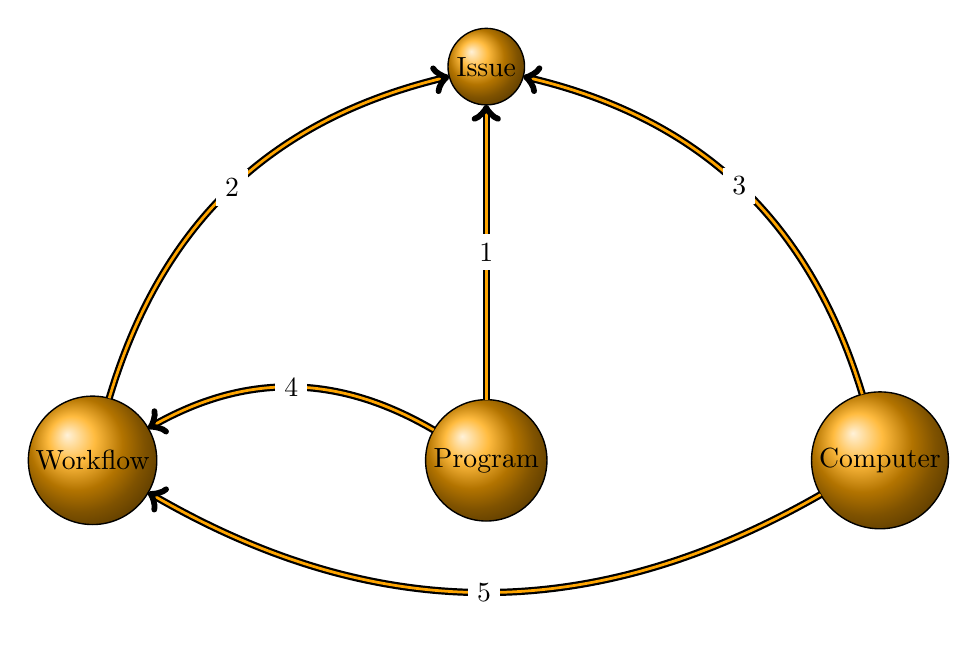
\begin{tikzpicture}
  	   	\GraphInit[vstyle = Shade]
  	   	\SetGraphUnit{5}
  	   	\Vertex{Issue}
  	   	\SOWE(Issue){Workflow}
  	   	\SO(Issue){Program}
  	   	\SOEA(Issue){Computer}
  	   	
  	   	
  	   	\Edge[label = 1, style={<-}](Issue)(Program)
  	   	\Edge[label = 2, style={<-,bend right}](Issue)(Workflow)
  	   	\Edge[label = 3, style={<-,bend left}](Issue)(Computer)
  	   	%\Edge[label = 4](Issue)(Computer)
  	   	%\Loop[dist = 4cm, dir = NO, label = 5](Computer.west)
  	   	%\Loop[dist = 4cm, dir = SO, label = 6](Program.east)
  	   	%\tikzset{EdgeStyle/.append style = {bend left = 50}}
  	   	\Edge[label = 4,style={<-,bend left}](Workflow)(Program)
  	   	\Edge[label = 5,style={->,bend left}](Computer)(Workflow)
  	   	%\Loop[dist = 4cm, dir = SOWE, label = 6](Program.west)
  	   \end{tikzpicture}}
  	\end{column}
  \end{columns}	
\end{frame}

%%%%%%%%%%%%%%%%%%%%%%%%%%%%%%%%%%%%%%%%%%%%%%%%%%%%%%%%%%%%%%%%%%%%%%%%%%%%%%%%
\begin{frame}
  \frametitle{What is the Nature of the Issue?}
  \texttt{Snakemake} helps you to identify the nature of an issue:
  \begin{enumerate}[<+->]
  	\item It will report to you in which \altverb{rule} the error occurred \textbf{and/or}
  	\item a so-called "traceback" to point the issue within its code.
  	\item The workflow will indicate log files on the screen.
  \end{enumerate}
  \pause
  \begin{docs}{Looking into Log Files}
  	Look into the log file. It \textit{should} tell you the error. \pause If not, report it to the workflow developer (next slides). 
  \end{docs}
\end{frame}

%%%%%%%%%%%%%%%%%%%%%%%%%%%%%%%%%%%%%%%%%%%%%%%%%%%%%%%%%%%%%%%%%%%%%%%%%%%%%%%%
\begin{frame}
  \frametitle{Do I need a \texttt{GitHub} account?}
  Today many software projects are either hosted on the global git server, \texttt{GitHub}.
  \begin{docs}
  	If you want to report an issue or even contribute back to the project, you will need an account. \lhref{https://docs.github.com/en/get-started/onboarding/getting-started-with-your-github-account}{This page} describes how. 
  \end{docs}
  
\end{frame}

%%%%%%%%%%%%%%%%%%%%%%%%%%%%%%%%%%%%%%%%%%%%%%%%%%%%%%%%%%%%%%%%%%%%%%%%%%%%%%%%
\begin{frame}
	\frametitle{Reporting Cluster Issues}
	\begin{question}[Where to?]
	  Report them to your cluster admins (\includegraphics[height=\texorpdfstring{\fontcharht\font`\B}]{logos/mattermost.png} chat, \Email{} mail ticket, etc.)
	\end{question}
    \pause
    \begin{question}[What?]
      Inaccessible paths (file system issue), network issues, node failures, etc. 
    \end{question}
    \pause
    \begin{question}[How?]
      Give a meaningful statement. "I can't do \altverb{ls} on \altverb{/some/path}." is more meaningful than "The filesystem stopped working!"\newline
      \bcattention Check your \Email{}! Has some maintenance been scheduled?
    \end{question}	
\end{frame}

%%%%%%%%%%%%%%%%%%%%%%%%%%%%%%%%%%%%%%%%%%%%%%%%%%%%%%%%%%%%%%%%%%%%%%%%%%%%%%%%
\begin{frame}
	\frametitle{Reporting Application Issues}
	\begin{question}[Where to?]
		The issue tracker of your application (if any). 
	\end{question}
	\pause
	\begin{question}[What?]
		Any application specific error. Try running the application with the input and parameters specified in the workflow (get them with \altverb{snakemake -p} to print the shell command or other debug flags). If the application breaks, report the failure. Else, it might be the workflow.
	\end{question}
	\pause
	\begin{question}[How?]
		Indicate the error message and what is leading to it. If you need special input to reproduce the issue, upload the input somewhere or attach minimal input to the issue report.
	\end{question}
\end{frame}

%%%%%%%%%%%%%%%%%%%%%%%%%%%%%%%%%%%%%%%%%%%%%%%%%%%%%%%%%%%%%%%%%%%%%%%%%%%%%%%%
\begin{frame}
	\frametitle{Reporting Workflow Issues}
	\begin{question}[Where to?]
		The issue tracker at your workflow. For \texttt{Snakemake} somewhere in the \lhref{https://snakemake.github.io/snakemake-workflow-catalog/}{catalog}. 
	\end{question}
	\pause
	\begin{question}[What?]
	   Check that it is you causing the error, e.\,g. undefined variables. \texttt{Snakemake} will inform you about the nature of the issue. Read the error output carefully. Report when sure it is not you.
	\end{question}
	\pause
	\begin{question}[How?]
		Indicate the error message and what is leading to it. If you need special input to reproduce the issue, upload the input somewhere or attach minimal input to the issue report.
	\end{question}
\end{frame}

%%%%%%%%%%%%%%%%%%%%%%%%%%%%%%%%%%%%%%%%%%%%%%%%%%%%%%%%%%%%%%%%%%%%%%%%%%%%%%%%
\begin{frame}
  \frametitle{Reporting \texttt{Snakemake} Issues}
  \begin{question}[Where to?]
  	 The \lhref{https://github.com/snakemake/snakemake/issues}{issue tracker of the \texttt{Snakemake} project}.
  \end{question}	
  \pause
  \begin{question}[What?]
  	Clearly unexpected behaviour. Or tracebacks pointing to \texttt{Snakemake} itself. 
  \end{question}
  \pause
  \begin{question}[How?]
  	Indicate the error message and what is leading to it (e.\,g. the command line you used). If you need special input to reproduce the issue, upload the input somewhere or attach minimal input to the issue report.
  \end{question}
\end{frame}

 
\end{document}

"
\ifdefined\ishandout
\PassOptionsToClass{handout}{beamer}
\fi

\documentclass[english,xcolor=pdftex,dvipsnames,aspectratio=<+++ if course.aspectratio is defined +++><++course.aspectratio++><+++else+++>43<+++endif+++>]{beamer} 

% to typeset only a few slide sets, set them here during development
%\includeonly{Why_Workflows}

\usepackage{etoolbox}
%\setbeamertemplate{mini frames}[box]
\usepackage{babel}
\usepackage[utf8]{inputenc}
\usepackage[T1]{fontenc}
\usepackage{amsfonts,amsmath,amssymb}
\usepackage{textgreek}
\usepackage{wrapfig}

\usepackage[load-configurations=binary,binary-units=true]{siunitx}
\usepackage[normalem]{ulem} % for strikethrough with \sout

\usepackage{color,colortbl}
\usepackage{upquote}

\definecolor{pblue}{RGB}{45,106,148}
\definecolor{pdarkblue}{RGB}{35,71,100}
\definecolor{plightblue}{RGB}{90,159,212}
\definecolor{pyellow}{RGB}{255,212,59}
\definecolor{pdarkyellow}{RGB}{255,188,41}
\definecolor{orange}{RGB}{255,165,0}
\definecolor{plightyellow}{RGB}{255,232,115}
\definecolor{pdarkgrey}{RGB}{100,100,100}
\definecolor{pgrey}{RGB}{153,153,153}
\definecolor{plightgrey}{RGB}{233,233,233}
\definecolor{plightgrey2}{RGB}{247,247,247}
\definecolor{pnavy}{RGB}{0,0,170}
\definecolor{BrickRed}{RGB}{150,22,11}
\definecolor{BlueViolet}{RGB}{138, 43, 226}
\definecolor{PineGreen}{RGB}{0, 51, 0}
\definecolor{light-gray}{gray}{0.95}

\definecolor{UniRot}{RGB}{193,0,42}
\definecolor{UniDunkelGrau}{RGB}{99,99,99}
\definecolor{UniHellGrau}{RGB}{172,172,172}

\definecolor{UrlColor}{rgb}{0,0.08,0.45}
\definecolor{links}{rgb}{0,0,0}

\usetheme{CambridgeUS} % Pittsburgh, CambridgeUS
\usecolortheme{beaver} %wolverine | crane | beaver | seahorse
\useinnertheme{rounded} 
\useoutertheme{default}
\usefonttheme{default}
%\setbeamercovered{transparent}
\setbeamertemplate{footline}[frame number]

% remove the navigation symbols
\setbeamertemplate{navigation symbols}{}

% side margins
\setbeamersize{text margin left=0.5cm, text margin right=0.5cm}

\setbeamercolor{structure}{fg=UniRot}% to modify  immediately all palettes
\setbeamercolor{title}{fg=UniRot}
\setbeamercolor{title in head/foot}{fg=UniRot}

\setbeamercolor{block title}{bg=UniRot!20,fg=darkred}
\setbeamercolor{block body}{fg=black, bg=plightgrey2}

% \setbeamercolor{block title}{fg=white,bg=orange}
\setbeamercolor{block title alerted}{fg=white,bg=UniRot}
\setbeamercolor{block title example}{fg=white,bg=PineGreen!80}


% enables two line cols in tabular envs
\newcommand{\specialcell}[2][c]{%
  \begin{tabular}[#1]{@{}c@{}}#2\end{tabular}}
\usepackage{subfig}
\usepackage{tikz}
\usetikzlibrary{arrows,shapes,backgrounds,positioning,shadows,decorations,trees,decorations.pathreplacing}
\usepackage{tkz-graph}

\usepackage{smartdiagram}


\addtobeamertemplate{footline}{}{%
\begin{tikzpicture}[remember picture,overlay]
\node[anchor=south west,yshift=2pt] at (current page.south west) {\includegraphics[height=0.8cm]{../images/logos/zdv_logo.png}};
\end{tikzpicture}}

\usepackage[tikz]{bclogo}
\newenvironment{task}[1][Task]{\bclogo[arrondi=0.1,logo=\bcoutil]{#1}}{\endbclogo}
\newenvironment{docs}[1][Documentation]{\bclogo[arrondi=0.1,logo=\bcplume]{#1}}{\endbclogo}
\newenvironment{hint}[1][Hint]{\bclogo[arrondi=0.1,logo=\bcinfo]{#1}}{\endbclogo}
\newenvironment{warning}[1][Warning]{\bclogo[arrondi=0.1,logo=\bcattention]{#1}}{\endbclogo}
% ``d/Definition'' is already defined ;-)
\newenvironment{explanation}[1][Definition]{\bclogo[arrondi=0.1,logo=\bcplume]{#1}}{\endbclogo}
\newenvironment{question}[1][Question]{\bclogo[arrondi=0.1,logo=\bcquestion]{#1}}{\endbclogo}


%%%%%%%%%%%%%%%%%
%% PLEASE NOTE %%
%%%%%%%%%%%%%%%%%
% frames containing ``Hand Out'' or ``Interlude'' should be started:

% \setcounter{preframe_handson}{\value{handson}}
% \begin{frame}[fragile]
%   \setcounter{handson}{\value{preframe_handson}}
%   \frametitle{\HandsOn{Using \texttt{find}}}

% or

% \setcounter{preframe_interlude}{\value{interlude}}
% \begin{frame}[fragile]
%   \setcounter{interlude}{\value{preframe_interlude}}
%   \frametitle{Interlude -- Parameter Extension}

% respectively.

\newcounter{handson}
\setcounter{handson}{1}
\newcounter{preframe_handson}
\setcounter{preframe_handson}{1}
\newcommand{\HandsOn}[1]{Hands On \Roman{handson} -- #1 \addtocounter{handson}{1}}
%\newcommand{\HandsOn}[1]{Hands On -- #1}

%TODO: Merge ``HandsOn'' && ``Excercise''
\newcounter{exercise}
\setcounter{exercise}{1}
% \newcommand{\Exercise}{\theexercise . Excercise \addtocounter{exercise}{1}}

% Bugfix of the Exercise command: avoid the annoying counter
\newcommand{\Exercise}{\theexercise . Excercise \addtocounter{exercise}{1}}

\newcounter{interlude}
\setcounter{interlude}{1}
\newcounter{preframe_interlude}
\setcounter{preframe_interlude}{1}

%\newcommand{\Interlude}[1]{Interlude \Roman{interlude} -- #1 \addtocounter{interlude}{1}}

% Bugfix of the Interlude command: avoid the annoying counter!
\newcommand{\Interlude}[1]{Interlude -- #1}

\usepackage{marvosym}
\usepackage{multicol}

\usepackage{hhline}

\usepackage{times}

% will decrease the font size for one frame
\newcommand\Fontvi{\fontsize{6}{7.2}\selectfont}
% 
\usepackage{dirtree,float} % for directory tree listings
\usepackage[nodisplayskipstretch]{setspace}


\usepackage{verbatim}
\usepackage{listings}

\newcommand{\altverb}[2][{}]{\colorbox{plightgrey}{\lstinline[language={#1}]{#2}}}


\lstloadlanguages{Python,bash,C++}
\lstset{showspaces=false,
basicstyle=\small,
showstringspaces=false}

\lstdefinestyle{tree}{
    literate=
    {├}{{smash{raisebox{-1ex}{rule{1pt}{baselineskip}}}raisebox{0.5ex}{rule{1ex}{1pt}}}}1 
    {─}{{raisebox{0.5ex}{rule{1.5ex}{1pt}}}}1 
    {└}{{smash{raisebox{0.5ex}{rule{1pt}{dimexprbaselineskip-1.5ex}}}raisebox{0.5ex}{rule{1ex}{1pt}}}}1 
  }

%default python listings:
\lstdefinestyle{Python}
{
  language=Python,
  basicstyle=\small,
  showstringspaces=false,
  stepnumber=5,
  numberstyle=\tiny,
  numbersep=5pt,
  showspaces=false,
  frame=single,
  framerule=0.4pt,
  rulecolor=\color{pgrey},
  backgroundcolor=\color{white},
  stringstyle=\color{BrickRed},
  keywordstyle=\color{BlueViolet}\bfseries,
  commentstyle=\color{PineGreen}\bfseries,
  identifierstyle={},
  emph={[10]self}, emphstyle={[10]\color{pblue}},
  emph={[11]yield}, emphstyle={[11]\color{pblue}},
  moredelim=**[is][\bfseries\color{red}]{@}{@},
  literate={\\@}{{\makeatletter @ \makeatother}}1
}

\lstdefinestyle{R}
{
  language=R,
  basicstyle=\small,
  showstringspaces=false,
  stepnumber=5,
  numberstyle=\tiny,
  numbersep=5pt,
  showspaces=false,
  frame=single,
  framerule=0.4pt,
  rulecolor=\color{pgrey},
  backgroundcolor=\color{white},
  stringstyle=\color{BrickRed},
  keywordstyle=\color{BlueViolet}\bfseries,
  commentstyle=\color{PineGreen}\bfseries,
  identifierstyle={},
  emph={[10]self}, emphstyle={[10]\color{pblue}},
  emph={[11]yield}, emphstyle={[11]\color{pblue}},
}

%default python listings:
\lstdefinestyle{C++}
{
  language=C++,
  basicstyle=\small,
  showstringspaces=false,
  stepnumber=5,
  numberstyle=\tiny,
  numbersep=5pt,
  showspaces=false,
  frame=single,
  framerule=0.4pt,
  rulecolor=\color{pgrey},
  backgroundcolor=\color{white},
  stringstyle=\color{BrickRed},
  keywordstyle=\color{BlueViolet}\bfseries,
  commentstyle=\color{PineGreen}\bfseries,
  identifierstyle={},
  emph={[10]self}, emphstyle={[10]\color{pblue}},
  emph={[11]yield}, emphstyle={[11]\color{pblue}},
}

\newcommand{\CC}{C\nolinebreak\hspace{-.05em}\raisebox{1ex}{\tiny\bf +}\nolinebreak\hspace{-.10em}\raisebox{1ex}{\tiny\bf +}}

%default shell listings:
\lstdefinestyle{Shell}
{
  language=Bash,
  basicstyle=\ttfamily\small,
  showstringspaces=false,
  frame=single,
  framerule=0.4pt,
  rulecolor=\color{pgrey},
  backgroundcolor=\color{plightgrey2},
  stringstyle=\color{BrickRed},
  keywordstyle=\color{BlueViolet},
  commentstyle=\color{PineGreen}\bfseries,
  identifierstyle=\color{black},
  emph={[10]\$,>>>}, emphstyle={[10]\color{pblue}},
  moredelim=**[is][\bfseries\color{red}]{@}{@},
  literate={\\@}{{\makeatletter @ \makeatother}}1
}

%default plain listings (e.g. for config files):https://www.google.com/search?client=firefox-b-e&q=conrad
\lstdefinestyle{Plain}
{ 
  stepnumber=5,
  numberstyle=\tiny,
  numbersep=5pt,
  language=Bash,
  basicstyle=\ttfamily\small,
  showstringspaces=false,
  frame=single,
  framerule=0.4pt,
  rulecolor=\color{pgrey},
  backgroundcolor=\color{plightgrey2},
  stringstyle=\color{black},
  keywordstyle=\color{black},
  commentstyle=\color{blue}\bfseries,
  identifierstyle=\color{black},
  breaklines=true,
  emph={[10]\$,>>>}, emphstyle={[10]\color{pblue}}
}

\lstdefinelanguage{XML}
{
  frame=single,
  framerule=0.4pt,
  rulecolor=\color{pgrey},
  backgroundcolor=\color{plightgrey2},
  stringstyle=\color{black},
  keywordstyle=\color{black},
  commentstyle=\color{blue}\bfseries,
  identifierstyle=\color{black},
  emph={[10]\$,>>>}, emphstyle={[10]\color{pblue}}
  morestring=[b]",
  morestring=[s]{>}{<},
  morecomment=[s]{<?}{?>},
  morekeywords={xmlns,version,type}% list your attributes here
}

\newcommand{\bibtex}{\textsc{Bib}\TeX}

%%% https://tex.stackexchange.com/questions/99316/symbol-for-external-links
\newcommand{\LinkSymbol}{%
  \tikz[x=1.2ex, y=1.2ex, baseline=-0.05ex]{% 
    \begin{scope}[x=1ex, y=1ex]
      \clip (-0.1,-0.1) 
      --++ (-0, 1.2) 
      --++ (0.6, 0) 
      --++ (0, -0.6) 
      --++ (0.6, 0) 
      --++ (0, -1);
      \path[draw, 
      line width = 0.5, 
      rounded corners=0.5] 
      (0,0) rectangle (1,1);
    \end{scope}
    \path[draw, line width = 0.5] (0.5, 0.5) 
    -- (1, 1);
    \path[draw, line width = 0.5] (0.6, 1) 
    -- (1, 1) -- (1, 0.6);
  }
}
\newcommand{\lhref}[2]{\href{#1}{#2\,\LinkSymbol}}

%%%% shortcuts for uniform appearance of common strings %%%%
\newcommand{\slurm}{\textsc{slurm}~}
\makeatletter
\newcommand{\rmnum}[1]{\romannumeral #1}
\newcommand{\Rmnum}[1]{\expandafter\@slowromancap\romannumeral #1@}
\makeatother

% this package provides the option to read parameters from a configuration file
\usepackage{readarray}

\readdef{config/config.dat}{\data}
\readarray\data\MyDat[-,3]
\newcommand\configparam[1]{\csname DATA#1\endcsname}
%\MyDatROWS{} rows of data read.

\newcounter{datacount}
\setcounter{datacount}{0}%
\whiledo{\value{datacount} < \MyDatROWS}{%
	\stepcounter{datacount}%
	\expandafter\xdef\csname DATA\MyDat[\arabic{datacount},1]\endcsname{%
		\MyDat[\arabic{datacount},3]}%
}



%\newcommand{\pathtoexercise}[1]{\path{/lustre/project/m2_jgu-ngstraing/workflows/#1}}
%\newcommand{\pathtoexercise}[1]{\path{ \DTLfetch{data}{thekey}{#1}{thevalue}   }}
%\newcommand{\pathtoclozure}[1]{\path{/lustre/project/hpckurs/bash-course/cloze/#1}}
%\newcommand{\pathtosolution}[1]{\path{/lustre/project/hpckurs/bash-course/solutions/#1}}

\setcounter{tocdepth}{1}

% this allows turning of footlines for particular slides
\setbeamertemplate{footline}[frame number]
% to use it, perform:

% \begin{frame}
% normal frame
% \end{frame}
% 
% \begingroup
% \setbeamertemplate{footline}{}
% \begin{frame}
% without footline
% \end{frame}
% \endgroup

%--------------------%
% Meta-Info 
%--------------------%



\title[Introduction to Workflow Programming]{An Introduction to HPC-conformant Scientific Workflows} 
%TODO: What should the subtitle be like? Should there be an Edition? How to keep track?
\subtitle{Workflow Course - Edition 3} 
\author[Snakemake Teaching Alliance]{The "Snakemake Teaching Alliance"}
% TODO: How do we insert a date, which is up to date? Should we insert one, here?
\date{September 2023}

\hypersetup{colorlinks,linkcolor=,urlcolor=links}

\graphicspath{{../images/}{../logos}}


% Passe captions an
\setbeamertemplate{caption}{\insertcaption}
% \setbeamerfont{caption}{size=\scriptsize}
\setlength\abovecaptionskip{-2.5pt}
\setlength\belowcaptionskip{0pt}



% For every picture that defines or uses external nodes, you'll have to
% apply the 'remember picture' style. To avoid some typing, we'll apply
% the style to all pictures.
\tikzstyle{every picture}+=[remember picture]
\tikzstyle{na} = [baseline=-.5ex]


\title[<++course.shorttitle++>]{<+++ if course.title is defined +++><++course.tittle++><+++else+++>Importance of \Snakemake Workflows for Admins and HPC-Users<+++endif+++>} 

\subtitle{<+++ if course.subtitle is defined +++><++course.subtitle++><+++else+++>Providing DataAnalytics Service<+++endif+++> - <++course.edition++>} 

%%%%%%%%%%%%%%%%%%%%%%%%%%%%%%%%%%%%%%%%%%%%%%%%%%%%%%%%%%%%%%%%%%%%%%%%%%%%%%%%
%%%%%%%%%%%%%%%%%%%%%%%%%%%%%%%%%%%%%%%%%%%%%%%%%%%%%%%%%%%%%%%%%%%%%%%%%%%%%%%%
\begin{document}
%%%%%%%%%%%%%%%%%%%%%%%%%%%%%%%%%%%%%%%%%%%%%%%%%%%%%%%%%%%%%%%%%%%%%%%%%%%%%%%%
%%%%%%%%%%%%%%%%%%%%%%%%%%%%%%%%%%%%%%%%%%%%%%%%%%%%%%%%%%%%%%%%%%%%%%%%%%%%%%%%

% attempts a better type setting for hboxes (might result in less overful warnings)
\sloppy

%%%%%%%%%%%%%%%%%%%%%%%%%%%%%%%%%%%%%%%%%%%%%%%%%%%%%%%%%%%%%%%%%%%%%%%%%%%%%%%% 
\begin{frame}[plain] % plain erzeugt Titelseite ohne Kopf- und Fußzeile
  \titlepage
\end{frame}

%%%%%%%%%%%%%%%%%%%%%%%%%%%%%%%%%%%%%%%%%%%%%%%%%%%%%%%%%%%%%%%%%%%%%%%%%%%%%%%%
\section{Why Workflows}

%%%%%%%%%%%%%%%%%%%%%%%%%%%%%%%%%%%%%%%%%%%%%%%%%%%%%%%%%%%%%%%%%%%%%%%%%%%%%%%%
\begin{frame}
    \frametitle{Outline}
    \begin{columns}[t]
        \begin{column}{.5\textwidth}
            \tableofcontents[sections={1-9},currentsection]
        \end{column}
        \begin{column}{.5\textwidth}
            \tableofcontents[sections={10-18},currentsection]
        \end{column}
    \end{columns}
\end{frame}

%%%%%%%%%%%%%%%%%%%%%%%%%%%%%%%%%%%%%%%%%%%%%%%%%%%%%%%%%%%%%%%%%%%%%%%%%%%%%%%%
\begin{frame}
  \frametitle{What is this about?}
   \begin{question}[Questions]
   	 \begin{itemize}
        \item I can code everything! Can I?
        \item What is the benefit of a workflow system?
        \item What distinguishes a workflow system from a ``pipeline''?
     \end{itemize}
   \end{question}
   \docs[Objectives]{\begin{enumerate}
                      \item Introducing workflow engines (particularly \texttt{Snakemake})!
                     \end{enumerate}}
\end{frame}  

%%%%%%%%%%%%%%%%%%%%%%%%%%%%%%%%%%%%%%%%%%%%%%%%%%%%%%%%%%%%%%%%%%%%%%%%%%%%%%%%
\begin{frame}
  \frametitle{Data Analysis}
  \begin{onlyenv}<1| handout:0>
    \begin{tikzpicture}
      \path[use as bounding box] (0.7,0) rectangle (12,8);
      \node[inner sep=0pt] (analysis_1) at (5,6)
         {\includegraphics[width=0.7\textwidth]{Snakemake/analysis_1.png}};   
      \node at (7, 3.5) %[below=-0.4cm of analysis_1, xshift=2.7cm] at (current page.center)
         {\includegraphics[width=0.45\textwidth]{Snakemake/phd_left.png}};
      \node at (6, 1) {\begin{minipage}{0.75\textwidth}\footnotesize
                        Idea from the official \lhref{https://slides.com/johanneskoester/snakemake-tutorial}{\texttt{Snakemake}} course (with permission), image from \lhref{https://phdcomics.com/comics.php}{PhD comics}.
                       \end{minipage}
      };
    \end{tikzpicture}    
  \end{onlyenv}
  
  \begin{onlyenv}<2| handout:1>
    \begin{tikzpicture}
      \path[use as bounding box] (0.7,0) rectangle (12,8);
      \node[inner sep=0pt] (analysis_full) at (5,6)
         {\includegraphics[width=0.7\textwidth]{Snakemake/analysis_full.png}};   
      \node at (7,3.5) % [below=-0.4cm of analysis_full, xshift=2.7cm]
         {\includegraphics[width=0.45\textwidth]{Snakemake/phd_full.png}};
      \node at (6, 1) {\begin{minipage}{0.75\textwidth}\footnotesize
                        Idea from the official \lhref{https://slides.com/johanneskoester/snakemake-tutorial}{\texttt{Snakemake}} course (with permission), image from \lhref{https://phdcomics.com/comics.php}{PhD comics}.
                       \end{minipage}
      };
    \end{tikzpicture}
  \end{onlyenv}
\end{frame}

%%%%%%%%%%%%%%%%%%%%%%%%%%%%%%%%%%%%%%%%%%%%%%%%%%%%%%%%%%%%%%%%%%%%%%%%%%%%%%%%
\begin{frame}
  \frametitle{Goals of Reproducibility}
  \Huge
  \begin{enumerate}
   \item Dispel Doubts
   \item Facilitate Further Experimentation
  \end{enumerate}
  \vfill
  \footnotesize{Idea from \lhref{https://elephly.net/downies/2023-dfn-slides.pdf}{DFN slides}.}
\end{frame}

%%%%%%%%%%%%%%%%%%%%%%%%%%%%%%%%%%%%%%%%%%%%%%%%%%%%%%%%%%%%%%%%%%%%%%%%%%%%%%%%
\begin{frame}
  \frametitle{Reproducible Data Analysis}
  \begin{onlyenv}<1| handout:0>
    \begin{tikzpicture}
      \path[use as bounding box] (0.7,0) rectangle (12,8);
      \node at (5.5, 5.5) {\includegraphics[width=0.7\textwidth]{Snakemake/automation.png}};
      \node at (8, 2.5) {\begin{minipage}{0.65\textwidth}
                             \textbf{From raw data to final figures:}
                             \begin{itemize}
                                \item \textbf{document} parameters, tools, versions
                                \item \textbf{execute} without manual intervention
                              \end{itemize}
                           \end{minipage}
                           };
    \end{tikzpicture}
  \end{onlyenv}
  \begin{onlyenv}<2| handout:0>
    \begin{tikzpicture}
      \path[use as bounding box] (0.7,0) rectangle (12,8);
      \node at (5.5, 5.5) {\includegraphics[width=0.7\textwidth]{Snakemake/scalability.png}};
      \node at (8, 2.5) {\begin{minipage}{0.65\textwidth}
                             \textbf{Handle parallelization:}
                             \begin{itemize}
                                \item execute for tens of thousands of datasets
                                \item efficiently use any computing platform
                              \end{itemize}
                           \end{minipage}
                           };
    \end{tikzpicture}
  \end{onlyenv}
  \begin{onlyenv}<3| handout:1>
    \begin{tikzpicture}
      \path[use as bounding box] (0.7,0) rectangle (12,8);
      \node at (5.5, 5.5) {\includegraphics[width=0.7\textwidth]{Snakemake/portability.png}};
      \node at (8, 2.5) {\begin{minipage}{0.65\textwidth}
                             \textbf{Handle deployment:}\newline
                             be able to easily execute analyses on a different system/platform/infrastructure
                           \end{minipage}
                           };
    \end{tikzpicture}
  \end{onlyenv}
\end{frame}

%%%%%%%%%%%%%%%%%%%%%%%%%%%%%%%%%%%%%%%%%%%%%%%%%%%%%%%%%%%%%%%%%%%%%%%%%%%%%%%%
\begin{frame}
  \frametitle{Beyond Reproducibility}
  \begin{onlyenv}<1| handout:0>
    \begin{figure}
      \centering
      \includegraphics[width=0.85\textwidth]{Snakemake/reproducibility_only.png}
    \end{figure}
  \end{onlyenv}
  \begin{onlyenv}<2| handout:0>
    \begin{figure}
      \centering
      \includegraphics[width=0.85\textwidth]{Snakemake/reproducibility_empty.png}
    \end{figure}
  \end{onlyenv}
  \begin{onlyenv}<3| handout:0>
    \begin{figure}
      \centering
      \includegraphics[width=0.85\textwidth]{Snakemake/reproducibility_left.png}
    \end{figure}
  \end{onlyenv}
    \begin{onlyenv}<4| handout:1>
      \begin{figure}
        \centering
        \includegraphics[width=0.85\textwidth]{Snakemake/reproducibility_full.png}
      \end{figure}
  \end{onlyenv}
\end{frame}

%%%%%%%%%%%%%%%%%%%%%%%%%%%%%%%%%%%%%%%%%%%%%%%%%%%%%%%%%%%%%%%%%%%%%%%%%%%%%%%%
\begin{frame}
  \frametitle{\textbf{Snakemake}}
  \begin{figure}
    \centering
    \caption{\textbf{>370k} downloads since 2015\newline
             \textbf{>1300} citations\newline
             \textbf{>7} citations per week since 2021}
    \includegraphics[width=0.6\textwidth]{Snakemake/paper_wall.png}
  \end{figure}
\end{frame}

%%%%%%%%%%%%%%%%%%%%%%%%%%%%%%%%%%%%%%%%%%%%%%%%%%%%%%%%%%%%%%%%%%%%%%%%%%%%%%%%
\begin{frame}
  \frametitle{The \includegraphics[width=2em]{logos/Snakemake.png} Catalogue}
  \begin{columns}
    \begin{column}{0.5\textwidth}
      \begin{itemize}[<+->]
   \item extremely feature rich
   \item over 1800 workflows in \lhref{https://snakemake.github.io/snakemake-workflow-catalog/}{its catalogue}
   \item almost a hundred standardized (meaning: will documented and with automatic deployment)
   \item cluster batch systems are supported (and support for various cloud systems, too)
   \item there is an option to include Nextflow wrappers, too.
      \end{itemize}
    \end{column}
    \begin{column}{0.5\textwidth}
      \begin{figure}
        \includegraphics[width=\textwidth]{Snakemake/Snakemake_Workflow_Catalog.png}
        \caption{Screenshot of the Workflow Catalogue}
      \end{figure}
    \end{column}
  \end{columns}
\end{frame}


%%%%%%%%%%%%%%%%%%%%%%%%%%%%%%%%%%%%%%%%%%%%%%%%%%%%%%%%%%%%%%%%%%%%%%%%%%%%%%%%
\subsection{Goals, Background \& Outline}

%%%%%%%%%%%%%%%%%%%%%%%%%%%%%%%%%%%%%%%%%%%%%%%%%%%%%%%%%%%%%%%%%%%%%%%%%%%%%%%%
\begin{frame}
  \frametitle{Questions}
  \begin{question}[The questions you most probably have when starting your Analysis:]
  	\begin{itemize}
      \item How to start quickly (with the lowest amount of overhead)?
      \item What are the necessary tools?
    \end{itemize}
  \end{question}
                                                                               
  \begin{question}[Our question to you:]
  	 How do you get this information? And: Is reproducibility and sustainability your concern?
  \begin{question}
  \pause
  \begin{block}{Most frequent Sources}
   \begin{itemize}
    \item Your labmate(s)
    \item The Internet
    \item Yes, of course ... eventually, when I brag about my paper/thesis.
   \end{itemize}
  \end{block}
\end{frame}

%%%%%%%%%%%%%%%%%%%%%%%%%%%%%%%%%%%%%%%%%%%%%%%%%%%%%%%%%%%%%%%%%%%%%%%%%%%%%%%%
\begin{frame}
  \frametitle{The Workflow Approach}
  Workflow Engines answer these questions directly by providing
  \begin{itemize}
   \item entire Workflows can be selected and can be put to action.
   \item executing routines reliably.
  \end{itemize}
\end{frame}

%%%%%%%%%%%%%%%%%%%%%%%%%%%%%%%%%%%%%%%%%%%%%%%%%%%%%%%%%%%%%%%%%%%%%%%%%%%%%%%%
\begin{frame}
  \frametitle{Going HPC}
  \begin{question}
  	Why would you want to work on a cluster?
  \end{question}
  \pause
  Answers may include:
  \begin{itemize}[<+->]
   \item compute power and ressources for big data
   \item launching scalable (and otherwise portable) workflows with workflow engines
  \end{itemize}
\end{frame}


%%%%%%%%%%%%%%%%%%%%%%%%%%%%%%%%%%%%%%%%%%%%%%%%%%%%%%%%%%%%%%%%%%%%%%%%%%%%%%%%
%%%%%%%%%%%%%%%%%%%%%%%%%%%%%%%%%%%%%%%%%%%%%%%%%%%%%%%%%%%%%%%%%%%%%%%%%%%%%%%%
\section{About Snakemake}
{   
	\usebackgroundtemplate{
		\vbox to \paperheight{\vfil\hbox to \paperwidth{\hfil\includegraphics[height=\paperheight]{logos/Wild_Python.jpg}\hfil}\vfil}
	}
	\frame{
		\frametitle{Snakemake}
		\begin{mdframed}[tikzsetting={draw=white,fill=white,fill opacity=0.8,
				line width=0pt},backgroundcolor=none,leftmargin=0,
			rightmargin=150,innertopmargin=4pt,roundcorner=10pt]
			\tableofcontents[currentsection,sections={1-4},hideothersubsections]
		\end{mdframed}
	}
}

%%%%%%%%%%%%%%%%%%%%%%%%%%%%%%%%%%%%%%%%%%%%%%%%%%%%%%%%%%%%%%%%%%%%%%%%%%%%%%%%
\begin{frame}
	\frametitle{What is this about?}
	\begin{question}[Questions]
		\begin{itemize}
			\item Why \Snakemake?
			\item Why not "Something Else"?
			\item Why Clusters?
		\end{itemize}
	\end{question}
	\begin{docs}[Objectives]
		\begin{enumerate}
			\item Introduction to \Snakemake Usage (in-depth will follow)
			\item Get an Mini-Overview about Workflow Systems
		\end{enumerate}
	\end{docs}
\end{frame}

\subsection{\Snakemake and the Workflow Catalogue}

%%%%%%%%%%%%%%%%%%%%%%%%%%%%%%%%%%%%%%%%%%%%%%%%%%%%%%%%%%%%%%%%%%%%%%%%%%%%%%%%
\begin{frame}
	\frametitle{\Snakemake}
	\begin{figure}
		\centering
		\caption*{\textbf{>1e6} downloads since 2015\newline
			\textbf{>1300} citations\newline
			\textbf{>7} citations per week since 2021}
		\includegraphics[width=0.6\textwidth]{Snakemake/paper_wall.png}
	\end{figure}
\end{frame}

%%%%%%%%%%%%%%%%%%%%%%%%%%%%%%%%%%%%%%%%%%%%%%%%%%%%%%%%%%%%%%%%%%%%%%%%%%%%%%%%
\begin{frame}
	\frametitle{\Snakemake is a NumFocus-Partner}
	\begin{columns}
		\begin{column}{0.5\textwidth}
			\includegraphics[width=.95\textwidth]{logos/NumFocus_LRG_WHITE-BG.png}
		\end{column}
	    \begin{column}{0.5\textwidth}
	    	\pause
	    	Partnered and in parts funded along projects like:
	    	\includegraphics[width=.95\textwidth]{logos/numfocus_projects.png}
	    \end{column}
	\end{columns}
\end{frame}

%%%%%%%%%%%%%%%%%%%%%%%%%%%%%%%%%%%%%%%%%%%%%%%%%%%%%%%%%%%%%%%%%%%%%%%%%%%%%%%%
\begin{frame}
	\frametitle{The \Snakemake{} Catalogue}
	\begin{columns}
		\begin{column}{0.5\textwidth}
			\begin{itemize}[<+->]
				\item Extremely feature rich: \lhref{https://snakemake.github.io/snakemake-workflow-catalog/}{over 1800 workflows}
				\item Almost a hundred standardized workflows ready to use (meaning: well documented and with automatic deployment)
				\item Cluster batch systems are supported (and support for various cloud systems, too)
				\item There is an option to include Nextflow wrappers, too.
			\end{itemize}
		\end{column}
		\begin{column}{0.5\textwidth}
			\begin{figure}
				\includegraphics[width=\textwidth]{Snakemake/Snakemake_Workflow_Catalog.png}
				\caption*{Screenshot of the Workflow Catalogue}
			\end{figure}
		\end{column}
	\end{columns}
\end{frame}

%%%%%%%%%%%%%%%%%%%%%%%%%%%%%%%%%%%%%%%%%%%%%%%%%%%%%%%%%%%%%%%%%%%%%%%%%%%%%%%%
\subsection{Background}

%%%%%%%%%%%%%%%%%%%%%%%%%%%%%%%%%%%%%%%%%%%%%%%%%%%%%%%%%%%%%%%%%%%%%%%%%%%%%%%%
\begin{frame}[fragile]
	\frametitle{How does \Snakemake on a Cluster work?}
	\begin{columns}[T]
		\begin{column}{.5\textwidth}
			\begin{itemize}[<+->]
				\item Snakemake is triggered on the command line:
				\begin{lstlisting}[language=Bash, style=Shell]
$ snakemake [<arguments>]
				\end{lstlisting} 
			    \item you will fill in the parameters of your workflow (in a file)
			    \item Snakemake will run on the login-node and spawn your jobs on the cluster 
			\end{itemize}
			
		\end{column}
		\begin{column}{.5\textwidth}
			\only<3>{\includegraphics[width=0.95\textwidth]{misc/cluster_scheme.png}}
		\end{column}
	\end{columns}
\end{frame}

%%%%%%%%%%%%%%%%%%%%%%%%%%%%%%%%%%%%%%%%%%%%%%%%%%%%%%%%%%%%%%%%%%%%%%%%%%%%%%%%
\begin{frame}<handout:0>
  \frametitle{"Spawn Jobs on a Cluster?!" - What does it mean?}
  \centering
  \begin{tabular}{m{0.1\textwidth} m{0.25\textwidth} m{0.2\textwidth} m{0.45\textwidth}}
PC: & \includegraphics[width=0.1\textwidth]{misc/pc_color.png}  	    &  \includegraphics[width=0.15\textwidth]{misc/sequential_code.png} &  \begin{minipage}{0.45\textwidth}
	$\Rightarrow$ sequential code \newline
	(perhaps parallel)
\end{minipage} \\ \pause
 	
Server: & \includegraphics[width=0.1\textwidth]{misc/homeserver.png}  	&  \includegraphics[width=0.15\textwidth]{misc/concurrent.pdf} & \begin{minipage}{0.45\textwidth}
	$\Rightarrow$ sequential code \newline(perhaps parallel), \newline some concurrency
	\end{minipage}\\ \pause
  	
Cluster: & \includegraphics[width=0.1\textwidth]{misc/data_center.png}  	&  \includegraphics[width=0.15\textwidth]{misc/high_concurrent.pdf} & \begin{minipage}{0.45\textwidth}
	$\Rightarrow$ programs launched \newline with high parallelism, \newline high concurreny
	\end{minipage}\\
  \end{tabular}
\end{frame}

%%%%%%%%%%%%%%%%%%%%%%%%%%%%%%%%%%%%%%%%%%%%%%%%%%%%%%%%%%%%%%%%%%%%%%%%%%%%%%%%
\begin{frame}
   \frametitle{Benefit of Cluster Usage}
   \begin{columns}
   	 \begin{column}{0.6\textwidth}
   	 	\centering
   	 	\includegraphics[width=0.8\textwidth]{workflows/molecular_screening_dag.jpeg}
   	 \end{column}
     \begin{column}{0.6\textwidth}
     	{\footnotesize
     		\Snakemake offers
     		\begin{itemize}[<+->]
     		  \item to carry out Nextflow wrappers
     		  \item to react on your input \newline $\Rightarrow$  more samples, more jobs
     		  \item to be a remedy to I/O contention
     		  \item to be ready for real time \newline computation with cluster support
     		  \item to support you from your input \newline to publication
     		  \item \ldots
     		\end{itemize}
     	}
     \end{column}
   \end{columns}
\end{frame}
	

%%%%%%%%%%%%%%%%%%%%%%%%%%%%%%%%%%%%%%%%%%%%%%%%%%%%%%%%%%%%%%%%%%%%%%%%%%%%%%%%
\section{Software Environment}

%%%%%%%%%%%%%%%%%%%%%%%%%%%%%%%%%%%%%%%%%%%%%%%%%%%%%%%%%%%%%%%%%%%%%%%%%%%%%%%%
\begin{frame}
	\frametitle{Outline}
	\begin{columns}[t]
		\begin{column}{.5\textwidth}
			\tableofcontents[sections={1-9},currentsection]
		\end{column}
		\begin{column}{.5\textwidth}
			\tableofcontents[sections={10-18},currentsection]
		\end{column}
	\end{columns}
\end{frame}


%%%%%%%%%%%%%%%%%%%%%%%%%%%%%%%%%%%%%%%%%%%%%%%%%%%%%%%%%%%%%%%%%%%%%%%%%%%%%%%%
\begin{frame}
	\frametitle{What is this about?}
	\question[Questions]{\begin{itemize}
			\item How do I get the software for a particular workflow?
			\item What is the difference in different build systems and software environments? Why does it matter for me?
		\end{itemize}
	}
	\docs[Objectives]{\begin{enumerate}
			\item Introducing the "Module" system provided on HPC clusters (briefly).
			\item Learning how to install software with "Conda".
			\item Knowing how to avoid conflicts between the different software provisioning schemes.
	\end{enumerate}}
\end{frame}  

%%%%%%%%%%%%%%%%%%%%%%%%%%%%%%%%%%%%%%%%%%%%%%%%%%%%%%%%%%%%%%%%%%%%%%%%%%%%%%%%
\subsection{Software on HPC Systems}

%%%%%%%%%%%%%%%%%%%%%%%%%%%%%%%%%%%%%%%%%%%%%%%%%%%%%%%%%%%%%%%%%%%%%%%%%%%%%%%% 
\begin{frame}
  \frametitle{Modules}
  \vspace{-1.3em}
  \begin{block}{What is a module?}
    A module collects all environment variables and settings needed for a particular software package (e.\,g. path to executable and libraries).
  \end{block}

  \vfill
\end{frame}

%%%%%%%%%%%%%%%%%%%%%%%%%%%%%%%%%%%%%%%%%%%%%%%%%%%%%%%%%%%%%%%%%%%%%%%%%%%%%%%%
\begin{frame}[fragile]
  {Modules -- Command Overview}
  \vspace{-1em}
  \begin{itemize}
    \setlength\itemsep{-0.1em}
  \item List of all available modules
    \begin{lstlisting}[language=Bash, style=Shell]
$ module avail             # or 'module av'
    \end{lstlisting}
  \item Loading a specific module
    \begin{lstlisting}[language=Bash, style=Shell]
$ module load <modulename> # or 'module add'
    \end{lstlisting}
  \item Showing all currently loaded modules
    \begin{lstlisting}[language=Bash, style=Shell]
$ module list
    \end{lstlisting}
  \item Unloading a specific module
    \begin{lstlisting}[language=Bash, style=Shell]
$ module unload <modulename>
    \end{lstlisting}
  \item Unload all active modules
    \begin{lstlisting}[language=Bash, style=Shell]
$ module purge
    \end{lstlisting}
  \end{itemize}
  \vfill
\end{frame}

%%%%%%%%%%%%%%%%%%%%%%%%%%%%%%%%%%%%%%%%%%%%%%%%%%%%%%%%%%%%%%%%%%%%%%%%%%%%%%%%
\begin{frame}[fragile]
  \frametitle{Modules -- looking for specific modules}
  Looking up modules:
  \begin{lstlisting}[language=Bash, style=Shell]
$ module spider <search string>
  \end{lstlisting}
  \pause
  \task[Looking for area specific modules]{Try looking for an area specific 
    module, e.\,g. in ``\texttt{bwa}''}
\end{frame}

%%%%%%%%%%%%%%%%%%%%%%%%%%%%%%%%%%%%%%%%%%%%%%%%%%%%%%%%%%%%%%%%%%%%%%%%%%%%%%%%
\begin{frame}[fragile]
   {Modules with easybuild\newline Or: What is this fuzz at the end of module names?}
   You will have seen modules like:
   \begin{lstlisting}[language=Bash, style=Shell]
numlib/FFTW/3.3.10-gompi-2021b   
   \end{lstlisting}
   \pause
   \begin{block}{Easybuild Naming Scheme}
    We are building our modules with \lhref{https://easybuilders.github.io/easybuild/}{easybuild} and adopted the following naming scheme for modules:\newline
    \footnotesize \verb+<topic>/<name>/<version>-<toolchain>-<toolchain-version>+
   \end{block}
   \pause
   \task[Look inside a module to know what will be loaded and set]{Do ``\texttt{module show <module>}''}
\end{frame}

%%%%%%%%%%%%%%%%%%%%%%%%%%%%%%%%%%%%%%%%%%%%%%%%%%%%%%%%%%%%%%%%%%%%%%%%%%%%%%%% 
\begin{frame}[fragile]
  \frametitle{That's all Folks}
   \vspace{-0.8em}
  \begin{alertblock}{Why we will not go in depth now}
You can learn more about modules in 101-HPC courses. Later, we will learn how to use \texttt{Snakemake} workflows, particularly curated ones, available on the web. We \emph{could} re-write and adapt them for Mogon, it is better to only parameterize them for Mogon and do leave the workflow itself unaltered. This is less cumbersome and as workflow systems, including \texttt{Snakemake}, rely on Conda, we will have an in-depth intro to Conda, instead.
  \end{alertblock}
  \vfill
  \begin{alertblock}{Do not mix Conda with Modules}
   Do not mix Conda with module files - particularly, avoid writing \altverb{module load} commands in your \texttt{\textasciitilde/.bashrc} file.\newline
   Whenever your modules or Conda are using conflicting compilers or environments, you might not be able to execute your software or -- \emph{worse} -- will result in funny crashes with apparently no reason.
  \end{alertblock}
\end{frame}

%%%%%%%%%%%%%%%%%%%%%%%%%%%%%%%%%%%%%%%%%%%%%%%%%%%%%%%%%%%%%%%%%%%%%%%%%%%%%%%% 
\subsection{Using Conda}

%%%%%%%%%%%%%%%%%%%%%%%%%%%%%%%%%%%%%%%%%%%%%%%%%%%%%%%%%%%%%%%%%%%%%%%%%%%%%%%% 
\begin{frame}<handout:0> 
  \frametitle{Your Work Environment with Conda}
  \begin{columns}
    \begin{column}{0.5\textwidth}\centering
      \includegraphics[width=0.8\textwidth]{environment/environment.png}
    \end{column}
    \begin{column}{0.5\textwidth}\centering
      \includegraphics[width=0.8\textwidth]{logos/Conda_logo.png}   
    \end{column}
  \end{columns}
\end{frame}

%%%%%%%%%%%%%%%%%%%%%%%%%%%%%%%%%%%%%%%%%%%%%%%%%%%%%%%%%%%%%%%%%%%%%%%%%%%%%%%% 
\begin{frame}
  \frametitle{Conda vs. Module Files}
  \begin{columns}
    \begin{column}{0.5\textwidth}
      Background Module Files
      \begin{itemize}
       \item module files provide an environment per software
       \item the software usually is compiled on the machine (optimized)
       \item due to differences in cluster naming schemes and setups portability cannot be granted
      \end{itemize}
    \end{column}
    \begin{column}{0.5\textwidth}
      Background Conda
      \begin{itemize}
       \item Conda is a machine independent package management systems
       \item packaged software is provided pre-compiled (NOT optimized)
       \item Conda allows for grouping software stacks in environments, therefore ensuring portability
      \end{itemize}
    \end{column}
  \end{columns}
\end{frame}


%%%%%%%%%%%%%%%%%%%%%%%%%%%%%%%%%%%%%%%%%%%%%%%%%%%%%%%%%%%%%%%%%%%%%%%%%%%%%%%% 
\begin{frame}[fragile]
  \frametitle{Installing Conda}
  You \emph{could} run
  \begin{lstlisting}[language=Bash, style=Shell, basicstyle=\small,breaklines=true ]
$ wget https://repo.anaconda.com/miniconda/Miniconda3-latest-Linux-x86_64.sh
  \end{lstlisting}
  to retrieve (Mini)Conda (a flavour of conda with less overhead).
  \hint{\footnotesize URL is from \url{https://docs.conda.io/en/latest/miniconda.html}.\newline However, we are going to use tweaked scripts provided to you.}
  \pause
  \hint{However, instead of downloading, we will work through this together on the slides to come.}
\end{frame} 

%%%%%%%%%%%%%%%%%%%%%%%%%%%%%%%%%%%%%%%%%%%%%%%%%%%%%%%%%%%%%%%%%%%%%%%%%%%%%%%% 
\begin{frame}[fragile]
  \frametitle{We will favour \emph{\textmu-Mamba} over Conda!}
  Everyone is knows ``Conda'' as a package manger -- and this is correct! But:
  \begin{block}{Why we recommend using ``\textmu-Mamba''}
   Conda carries some overhead. Alternative implementations can be faster and require less files. Mamba is a ``drop-in'' for Conda. This means: \emph{every command is the same}, except we will write \altverb{mamba} where usuall \altverb{conda} would be.\newline
   Why?\newline
   Mamba is an implementation of Conda, written in \CC{}. It is able to carry out some tasks in parallel and works considerably faster. In turn, \textmu-Mamba is a statically compiled version of Mamba and does not require a ``base'' environment (we will learn about environments, soon), which means even less overhead.
  \end{block}
\end{frame}

% %%%%%%%%%%%%%%%%%%%%%%%%%%%%%%%%%%%%%%%%%%%%%%%%%%%%%%%%%%%%%%%%%%%%%%%%%%%%%%%% 
% \begin{frame}[fragile]
%   \frametitle{\HandsOn{Copy our Course Sample Data}}
%   We shall copy a few install scripts (which also will download some sample data).\newline
%   Please copy \pathtoexercise.\newline
%   \begin{lstlisting}[language=Bash, style=Shell]
% $ # Hint: This is the general syntax:
% $ cp -r <path> ~/.
%   \end{lstlisting}
%   \hint[Note]{The slides assume that you are working in your HOME. Then typing the \textasciitilde{} is not necessary.}
% \end{frame}
% 
% %%%%%%%%%%%%%%%%%%%%%%%%%%%%%%%%%%%%%%%%%%%%%%%%%%%%%%%%%%%%%%%%%%%%%%%%%%%%%%%% 
% \begin{frame}[fragile]
%   \frametitle{\Interlude{About working with \texttt{Snakefile} Templates}}
%   \begin{block}{\texttt{Snakefile} Templates}
%    Your copied folder contains a folder ``\texttt{Template\_Snakefiles}''. Instead of typing workflows, we will refer to this folder, from where you can copy templates or cloze texts.
%   \end{block}
%   \begin{exampleblock}{Working with \texttt{Snakefile}s}
%    \texttt{Snakemake} expexts a worflow file named \texttt{Snakefile}. When you copy a template, e.\,g. \altverb{01_Snakefile}, you best proceed with these steps:
%    \begin{lstlisting}[language=Bash, style=Shell,basicstyle=\footnotesize]
% $ cp ~/worflows/Template_Snakefiles/01_Snakefile Snakefile
%    \end{lstlisting}
%   \end{exampleblock}
% \end{frame}



 
% %%%%%%%%%%%%%%%%%%%%%%%%%%%%%%%%%%%%%%%%%%%%%%%%%%%%%%%%%%%%%%%%%%%%%%%%%%%%%%%% 
% \begin{frame}[fragile]
%   \frametitle{The Install Script}
%   The install script reads:
%   \begin{lstlisting}[language=Bash, style=Shell]
% # 1. download mamba-forge
% echo "downloading Mambaforge"
% curl -L https://github.com/conda-forge/miniforge/releases/latest/download/Mambaforge-Linux-x86_64.sh -o Mambaforge-Linux-x86_64.sh
% 
% # 2. inform the user that all requests have to be confirmed
% echo "going to install Mambaforge. Please confirm all questions with 'yes'"
% sleep 2
% 
% # 3. starting the installation process
% bash Mambaforge-Linux-x86_64.sh
%   \end{lstlisting}
%   Basically, download \& install - any questions?
% \end{frame}

%%%%%%%%%%%%%%%%%%%%%%%%%%%%%%%%%%%%%%%%%%%%%%%%%%%%%%%%%%%%%%%%%%%%%%%%%%%%%%%% 
\begin{frame}[fragile]
  \frametitle{Installing \sout{Conda}/\textmu-Mamba - IV}
  \footnotesize
  \begin{columns}[t]
    \begin{column}{0.5\textwidth}
       You now have a section like this in your ``\texttt{\textasciitilde/.bashrc}'':
       \begin{lstlisting}[language=Bash, style=Shell, basicstyle=\tiny, breaklines=true]
# >>> mamba initialize >>>
# !! Contents within this block are managed by 'mamba init' !!
export MAMBA_EXE='/home/cm/.local/bin/micromamba';
export MAMBA_ROOT_PREFIX='/home/cm/micromamba';
__mamba_setup="$("$MAMBA_EXE" shell hook --shell bash --root-prefix "$MAMBA_ROOT_PREFIX" 2> /dev/null)"
if [ $? -eq 0 ]; then
    eval "$__mamba_setup"
else
    alias micromamba="$MAMBA_EXE"  # Fallback on help from mamba activate
fi
unset __mamba_setup
# <<< mamba initialize <<<
      \end{lstlisting}
      \bcattention \emph{Every} time you log-in this will be executed. Also, here, ``\texttt{<prefix>}'' denotes \emph{your} prefix.
    \end{column}
    \begin{column}{0.5\textwidth}
       \pause
       Please edit your ``\texttt{\textasciitilde/.bashrc}'' file and put part in a function, to re-gain manual control:
       \begin{lstlisting}[language=Bash, style=Shell, basicstyle=\tiny, breaklines=true]
@function conda_initialize {@
# >>> mamba initialize >>>
# !! Contents within this block are managed by 'mamba init' !!
export MAMBA_EXE='/home/cm/.local/bin/micromamba';
export MAMBA_ROOT_PREFIX='/home/cm/micromamba';
__mamba_setup="$("$MAMBA_EXE" shell hook --shell bash --root-prefix "$MAMBA_ROOT_PREFIX" 2> /dev/null)"
if [ $? -eq 0 ]; then
    eval "$__mamba_setup"
else
    alias micromamba="$MAMBA_EXE"  # Fallback on help from mamba activate
fi
unset __mamba_setup
# <<< mamba initialize <<<
@}@
      \end{lstlisting}
      \bcattention Add the highlighted lines! and your login will be faster! Also, this allows to separate the module environment and conda-related environments safely.
    \end{column}
  \end{columns}
\end{frame}

%%%%%%%%%%%%%%%%%%%%%%%%%%%%%%%%%%%%%%%%%%%%%%%%%%%%%%%%%%%%%%%%%%%%%%%%%%%%%%%% 
\begin{frame}[fragile]
  \frametitle{Why this function in your \texttt{.bashrc}?}
  \begin{itemize}[<+->]
  		\item \emph{every} time you log in, the code in your \texttt{.bashrc} will be exectud. Depeding on your conda setup, this can be incredebly slow (another reason to use Mamba or \textmu-Mamba).
  		\item automatic inclusion of Conda/Mamba might cause interference with modules
  		\item Now, you can run \verb+conda_initialize+ in the login shell, jobs scripts, etc. upon demand and deactivate if needed.
  	\end{itemize}
\end{frame}

%%%%%%%%%%%%%%%%%%%%%%%%%%%%%%%%%%%%%%%%%%%%%%%%%%%%%%%%%%%%%%%%%%%%%%%%%%%%%%%% 
\begin{frame}[fragile]
  \frametitle{Initializing Conda \& Mamba}
  To initialize Conda, simply run
  \begin{lstlisting}[language=Bash, style=Shell]
$ bash
  \end{lstlisting}
  or (better)
  \begin{lstlisting}[language=Bash, style=Shell]
$ source ~/.bashrc
$ conda_initialize # if you have this function
  \end{lstlisting}
\end{frame}


%%%%%%%%%%%%%%%%%%%%%%%%%%%%%%%%%%%%%%%%%%%%%%%%%%%%%%%%%%%%%%%%%%%%%%%%%%%%%%%% 
\begin{frame}[fragile]
  \frametitle{Reducing Search Overhead - the \texttt{.condarc}-File}
  On \mogon{} the number of Conda channels (the repositories) is reduced by the whitelisting. Nevertheless, it helps to reduce the search time with a resource file, including  a number of definitions, \emph{before} starting:
  \begin{lstlisting}[language=Bash, style=Shell, basicstyle=\tiny]
$ cat .condarc
create_default_packages:
  - setuptools
channels:
  - conda-forge
  - bioconda
  - defaults
  - r
proxy_servers:
  http: http://webproxy.zdv.uni-mainz.de:8888
ssl_verify: false
auto_update_conda: false
always_yes: true # avoid confirmation(s)
  \end{lstlisting}
  To obtain the same resource file, run:
  \begin{lstlisting}[language=Bash, style=Shell, basicstyle=\footnotesize]
$ cp ../setup/condarc ~/.condarc
  \end{lstlisting}
  More on \altverb{.condarc} on the \lhref{https://conda.io/projects/conda/en/latest/user-guide/configuration/use-condarc.html}{official Conda documentation site}
\end{frame}

%%%%%%%%%%%%%%%%%%%%%%%%%%%%%%%%%%%%%%%%%%%%%%%%%%%%%%%%%%%%%%%%%%%%%%%%%%%%%%%% 
\begin{frame}[fragile]
  \frametitle{Searching Software with Conda v. Mamba}
  First you might want to look for software. This is done with
  \begin{lstlisting}[language=Bash, style=Shell]
$ micromamba search <softwarename>
  \end{lstlisting}
  \pause
  \task{Try this with a software which comes to mind.}
  \pause
  This will list packages with channel and version information, e.\,g.
  \begin{lstlisting}[language=Bash, style=Shell, basicstyle=\tiny]
$ mamba search minimap
<snip>
Loading channels: done
# Name                       Version           Build  Channel             
minimap                     0.2_r124               0  bioconda            
minimap                     0.2_r124      h5bf99c6_4  bioconda
....
  \end{lstlisting}
\end{frame}


%%%%%%%%%%%%%%%%%%%%%%%%%%%%%%%%%%%%%%%%%%%%%%%%%%%%%%%%%%%%%%%%%%%%%%%%%%%%%%%% 
\begin{frame}[fragile]
  \frametitle{Installing Software \emph{with} Conda \& Mamba - Using Environments}
  \hint{It is a good habit to have
        \begin{itemize}
          \item \emph{an} environment per workflow
          \item the environment named as the workflow
          \item this way, we have a bundle of tools, activate the environment for it
          \item \texttt{snakemake} workflows will install the tools you need for a particular workflow - only \emph{if} these tools are still missing
         \end{itemize}
        }
\end{frame}


%%%%%%%%%%%%%%%%%%%%%%%%%%%%%%%%%%%%%%%%%%%%%%%%%%%%%%%%%%%%%%%%%%%%%%%%%%%%%%%% 
\begin{frame}[fragile]
  \frametitle{Conda Environments}
  With Conda/Mamba, we can activate and deactivate environments, which bundle our software. E.\,g. a software stack per workflow to ensure reproducible runs.
    \pause
  To generate a new we can run
  \begin{lstlisting}[language=Bash, style=Shell]
$ micromamba create --pyc -f environment.txt -p /lustre/project/m2_zdvhpc/meesters/test_micromamba
$ mamba info --envs
  \end{lstlisting}
  We can create, activate and deactivate environments with
  \begin{lstlisting}[language=Bash, style=Shell]
$ mamba create --name <environment name>
$ mamba activate <environment name>
$ mamba deactivate
  \end{lstlisting}
\end{frame}






%%%%%%%%%%%%%%%%%%%%%%%%%%%%%%%%%%%%%%%%%%%%%%%%%%%%%%%%%%%%%%%%%%%%%%%%%%%%%%%%
\include{admin/actual_work}

%%%%%%%%%%%%%%%%%%%%%%%%%%%%%%%%%%%%%%%%%%%%%%%%%%%%%%%%%%%%%%%%%%%%%%%%%%%%%%%%
%%%%%%%%%%%%%%%%%%%%%%%%%%%%%%%%%%%%%%%%%%%%%%%%%%%%%%%%%%%%%%%%%%%%%%%%%%%%%%%%
\section{Parametizing your Workflow - II}

%%%%%%%%%%%%%%%%%%%%%%%%%%%%%%%%%%%%%%%%%%%%%%%%%%%%%%%%%%%%%%%%%%%%%%%%%%%%%%%%
\begin{frame}
    \frametitle{Outline}
    \begin{columns}[t]
        \begin{column}{.5\textwidth}
            \tableofcontents[sections={1-9},currentsection]
        \end{column}
        \begin{column}{.5\textwidth}
            \tableofcontents[sections={10-18},currentsection]
        \end{column}
    \end{columns}
\end{frame}

%%%%%%%%%%%%%%%%%%%%%%%%%%%%%%%%%%%%%%%%%%%%%%%%%%%%%%%%%%%%%%%%%%%%%%%%%%%%%%%%
\begin{frame}
  \frametitle{What is this about?}
  \begin{question}[Questions]
   	\begin{itemize}
      \item How do we add execution parameters?
      \item How do we tune scientific parameters?
    \end{itemize}
  \end{question}
   \begin{docs}[Objectives]
   	 \begin{enumerate} 
        \item Learn to use parameters relevant for the batch systems.
        \item Learn how to tune \Snakemake{} on the command line.
        \item Learn how to tune \Snakemake{} with configuration files.
    \end{enumerate}
  \end{docs}
\end{frame}

%%%%%%%%%%%%%%%%%%%%%%%%%%%%%%%%%%%%%%%%%%%%%%%%%%%%%%%%%%%%%%%%%%%%%%%%%%%%%%%%
\subsection{The Configuration File}

%%%%%%%%%%%%%%%%%%%%%%%%%%%%%%%%%%%%%%%%%%%%%%%%%%%%%%%%%%%%%%%%%%%%%%%%%%%%%%%%
\begin{frame}[fragile]
	\frametitle{The \texttt{Snakemake} \texttt{resources} Section}
	\texttt{Snakemake} rules provide an additional \altverb{resource} section:
	\begin{lstlisting}[language=Python,style=Python]
rule <name>:
	...
	resources:
		partition='parallel',
		mem_mb=1800,
		cpus_per_task=4
	\end{lstlisting}
	\begin{hint}
		Note the \textbf{,}!
	\end{hint}
	\pause
	\begin{docs}
		You \emph{may} define \emph{any} resource keyword within any rule.
	\end{docs}
\end{frame}

%%%%%%%%%%%%%%%%%%%%%%%%%%%%%%%%%%%%%%%%%%%%%%%%%%%%%%%%%%%%%%%%%%%%%%%%%%%%%%%%
\begin{frame}
	\frametitle{The \texttt{Snakemake} \texttt{resources} Section - its Downside}
	\begin{block}{Every Resource Spec needs a Change per Rule???}
		You might have noticed, this specification per rule is most untidy. \texttt{Snakemake}'s design principle is: ship workflows which run \emph{everywhere} \& \emph{every time}.
		\newline \pause
		Relax: Every parameter can be specified:
		\begin{itemize}
			\item in a \texttt{Snakefile},
			\item on the command line,
			\item and re-usable in configuration files!
		\end{itemize}
	\end{block}
\end{frame}

%%%%%%%%%%%%%%%%%%%%%%%%%%%%%%%%%%%%%%%%%%%%%%%%%%%%%%%%%%%%%%%%%%%%%%%%%%%%%%%%
\begin{frame}[label=random]
	\frametitle{What is Random Access?}
	\vspace{-1.5em}
	\begin{figure}
		\centering
		\begin{tikzpicture}
			\node[name=sa] at (3.5,10) { \lhref{https://en.wikipedia.org/wiki/Random_access}{Sequential Access} };
			\foreach[count=\y from 2] \x in {1,...,11}{
				\draw[thick,black,midway,draw] (\x,8.75) rectangle node[name=s\x] {} (\y,8.25);
			}       
			\foreach[count=\y from 2] \x in  {1, ..., 10} {
					\path[->] ([yshift=.6em]s\x.north west) edge[bend left=30] ([yshift=.6em]s\y.north west);
			}
			%         \path[->] ([yshift=.6em]s1.north) edge [bend left=30] ([yshift=.6em]s2.north) ;
			
			\node[name=ra] at (3.5,7) { Random Access };
			\foreach[count=\y from 2] \x in {1,...,11}{
				\draw[thick,black,midway,draw] (\x,5.75) rectangle node[name=r\x] {} (\y,5.25);
			}
		
			\path[->] ([yshift=.6em]r1.north) edge [bend left=30] ([yshift=.6em]r5.north) ;
			\path[->] ([yshift=.6em]r5.north) edge [bend right=60] ([yshift=.6em]r2.north) ;
			\path[->] ([yshift=.6em]r2.north) edge [bend left=30] ([yshift=.6em]r3.north) ;
			\path[->] ([yshift=.6em]r3.north) edge [bend left=30] ([yshift=.6em]r11.north) ;
			\path[->] ([yshift=.6em]r11.north) edge [bend right=30] ([yshift=.6em]r7.north) ;
			\path[->] ([yshift=.6em]r7.north) edge [bend right=30] ([yshift=.6em]r6.north) ;
			\path[->] ([yshift=.6em]r6.north) edge [bend left=60] ([yshift=.6em]r8.north) ;
			\path[->] ([yshift=.6em]r8.north) edge [bend right=50] ([yshift=.6em]r4.north) ;
		\end{tikzpicture}
	\end{figure}
\end{frame}


\begin{frame}
	\frametitle{Upcoming Courses}
	\begin{columns}[T]
		\begin{column}{0.5\textwidth}
			\centering
			\includegraphics[width=0.7\textwidth]{humor/announcement.png}
			\caption{Me, announcing courses}
		\end{column}
	
	\begin{column}{0.5\textwidth}
		Do you want to learn:
		\begin{itemize}
			\item How to create \& publish \Snakemake workflows suitable for HPC clusters?
			\item Learn how to deploy and adapt $3^{\mathsf{rd}}$-party workflows?
			\item and more \ldots
		\end{itemize}
	    Check out these courses in
	    \begin{itemize}
	    	\item \lhref{https://indico.zdv.uni-mainz.de/event/23/}{Mainz, 29. \& 30. Jan.}
	    	\item \lhref{https://tu-dresden.de/zih/hochleistungsrechnen/nhr-training/bd-hpda/snakemake?set_language=en}{Dresden, 26. \& 27. Feb.}
	    \end{itemize}
	\end{column}
	
	\end{columns}
\end{frame}
      
%%%%%%%%%%%%%%%%%%%%%%%%%%%%%%%%%%%%%%%%%%%%%%%%%%%%%%%%%%%%%%%%%%%%%%%%%%%%%%%%
%\include{admin/Data_Management}

%%%%%%%%%%%%%%%%%%%%%%%%%%%%%%%%%%%%%%%%%%%%%%%%%%%%%%%%%%%%%%%%%%%%%%%%%%%%%%%%
% %%%%%%%%%%%%%%%%%%%%%%%%%%%%%%%%%%%%%%%%%%%%%%%%%%%%%%%%%%%%%%%%%%%%%%%%%%%%%%%%
\section{Contributing}

%%%%%%%%%%%%%%%%%%%%%%%%%%%%%%%%%%%%%%%%%%%%%%%%%%%%%%%%%%%%%%%%%%%%%%%%%%%%%%%%
\begin{frame}
	\frametitle{Outline}
	\begin{columns}[t]
		\begin{column}{.5\textwidth}
			\tableofcontents[sections={1-9},currentsection]
		\end{column}
		\begin{column}{.5\textwidth}
			\tableofcontents[sections={10-18},currentsection]
		\end{column}
	\end{columns}
\end{frame}

%%%%%%%%%%%%%%%%%%%%%%%%%%%%%%%%%%%%%%%%%%%%%%%%%%%%%%%%%%%%%%%%%%%%%%%%%%%%%%%%
\begin{frame}
	\frametitle{What is this about?}
	\begin{question}[Questions]
		\begin{itemize}
			\item How do I report Issues?
			\item How do I improve the Documentation?
		\end{itemize}
	\end{question}
	\begin{docs}[Objectives]
		\begin{enumerate}
			\item Learn how to figure out where an error comes from.
			\item Learning how to create a \emph{meaningful} issue report.
			\item Getting to know \texttt{GitHub}.
		\end{enumerate}
	\end{docs}
\end{frame}

%%%%%%%%%%%%%%%%%%%%%%%%%%%%%%%%%%%%%%%%%%%%%%%%%%%%%%%%%%%%%%%%%%%%%%%%%%%%%%%%
\begin{frame}
  \frametitle{"I am not a Programmer!"}
  \ldots and do not know what and how to contribute!
  \pause
  \begin{block}{Open Source is \emph{NOT JUST} about Programming}
  	\lhref{https://opensource.guide/how-to-contribute/}{You can contribute by}
  	\begin{itemize}[<+->]
  		\item writing whats wrong (issue reports)
  		\item writing how it's done (documentation)
  		\item organizing events (bringing people together)
  		\item checking (test the code submissions of other's)
  		\item etc. etc. etc.
  	\end{itemize}
  \end{block} 
\end{frame}

%%%%%%%%%%%%%%%%%%%%%%%%%%%%%%%%%%%%%%%%%%%%%%%%%%%%%%%%%%%%%%%%%%%%%%%%%%%%%%%%
\subsection{The Multitute of Issues}

%%%%%%%%%%%%%%%%%%%%%%%%%%%%%%%%%%%%%%%%%%%%%%%%%%%%%%%%%%%%%%%%%%%%%%%%%%%%%%%%
\begin{frame}
  \frametitle{Is it \texttt{Snakemake}, the Workflow or the Cluster?}
  	\begin{columns}[t]
  	\begin{column}{.5\textwidth}
  	  A workflow may break for a number of reasons:
  	  \begin{enumerate}
  	  	\item a program breaks
  	  	\item the workflow has an issue
  	  	\item a computer failure
  	  	\item a program version change breaks the workflow
  	  	\item some computer issue (e.\,g. disk failure) breaks the workflow
  	  \end{enumerate}
  	\end{column}
  	\begin{column}{.5\textwidth}
  	  \tikzset{
  	  	LabelStyle/.style = { rectangle, rounded corners, draw,
  	  		minimum width = 2em, fill = yellow!50,
  	  		text = red, font = \bfseries },
  	  	VertexStyle/.append style = { inner sep=5pt,
  	  		font = \Large\bfseries},
  	  	EdgeStyle/.append style = {->, bend left} }
    	\resizebox{\columnwidth}{!}{
  	   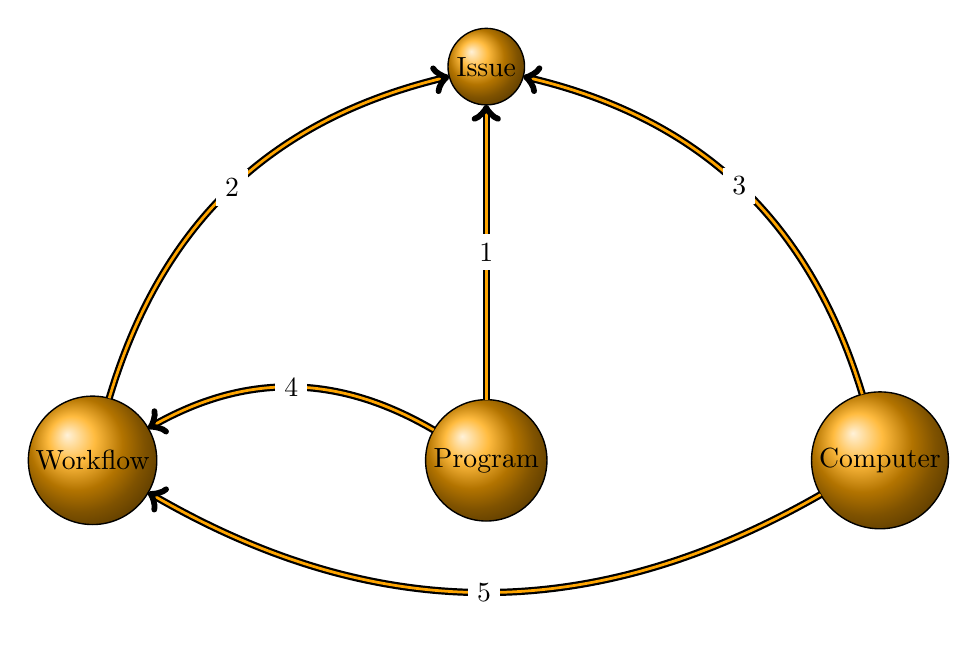
\begin{tikzpicture}
  	   	\GraphInit[vstyle = Shade]
  	   	\SetGraphUnit{5}
  	   	\Vertex{Issue}
  	   	\SOWE(Issue){Workflow}
  	   	\SO(Issue){Program}
  	   	\SOEA(Issue){Computer}
  	   	
  	   	
  	   	\Edge[label = 1, style={<-}](Issue)(Program)
  	   	\Edge[label = 2, style={<-,bend right}](Issue)(Workflow)
  	   	\Edge[label = 3, style={<-,bend left}](Issue)(Computer)
  	   	%\Edge[label = 4](Issue)(Computer)
  	   	%\Loop[dist = 4cm, dir = NO, label = 5](Computer.west)
  	   	%\Loop[dist = 4cm, dir = SO, label = 6](Program.east)
  	   	%\tikzset{EdgeStyle/.append style = {bend left = 50}}
  	   	\Edge[label = 4,style={<-,bend left}](Workflow)(Program)
  	   	\Edge[label = 5,style={->,bend left}](Computer)(Workflow)
  	   	%\Loop[dist = 4cm, dir = SOWE, label = 6](Program.west)
  	   \end{tikzpicture}}
  	\end{column}
  \end{columns}	
\end{frame}

%%%%%%%%%%%%%%%%%%%%%%%%%%%%%%%%%%%%%%%%%%%%%%%%%%%%%%%%%%%%%%%%%%%%%%%%%%%%%%%%
\begin{frame}
  \frametitle{What is the Nature of the Issue?}
  \texttt{Snakemake} helps you to identify the nature of an issue:
  \begin{enumerate}[<+->]
  	\item It will report to you in which \altverb{rule} the error occurred \textbf{and/or}
  	\item a so-called "traceback" to point the issue within its code.
  	\item The workflow will indicate log files on the screen.
  \end{enumerate}
  \pause
  \begin{docs}{Looking into Log Files}
  	Look into the log file. It \textit{should} tell you the error. \pause If not, report it to the workflow developer (next slides). 
  \end{docs}
\end{frame}

%%%%%%%%%%%%%%%%%%%%%%%%%%%%%%%%%%%%%%%%%%%%%%%%%%%%%%%%%%%%%%%%%%%%%%%%%%%%%%%%
\begin{frame}
  \frametitle{Do I need a \texttt{GitHub} account?}
  Today many software projects are either hosted on the global git server, \texttt{GitHub}.
  \begin{docs}
  	If you want to report an issue or even contribute back to the project, you will need an account. \lhref{https://docs.github.com/en/get-started/onboarding/getting-started-with-your-github-account}{This page} describes how. 
  \end{docs}
  
\end{frame}

%%%%%%%%%%%%%%%%%%%%%%%%%%%%%%%%%%%%%%%%%%%%%%%%%%%%%%%%%%%%%%%%%%%%%%%%%%%%%%%%
\begin{frame}
	\frametitle{Reporting Cluster Issues}
	\begin{question}[Where to?]
	  Report them to your cluster admins (\includegraphics[height=\texorpdfstring{\fontcharht\font`\B}]{logos/mattermost.png} chat, \Email{} mail ticket, etc.)
	\end{question}
    \pause
    \begin{question}[What?]
      Inaccessible paths (file system issue), network issues, node failures, etc. 
    \end{question}
    \pause
    \begin{question}[How?]
      Give a meaningful statement. "I can't do \altverb{ls} on \altverb{/some/path}." is more meaningful than "The filesystem stopped working!"\newline
      \bcattention Check your \Email{}! Has some maintenance been scheduled?
    \end{question}	
\end{frame}

%%%%%%%%%%%%%%%%%%%%%%%%%%%%%%%%%%%%%%%%%%%%%%%%%%%%%%%%%%%%%%%%%%%%%%%%%%%%%%%%
\begin{frame}
	\frametitle{Reporting Application Issues}
	\begin{question}[Where to?]
		The issue tracker of your application (if any). 
	\end{question}
	\pause
	\begin{question}[What?]
		Any application specific error. Try running the application with the input and parameters specified in the workflow (get them with \altverb{snakemake -p} to print the shell command or other debug flags). If the application breaks, report the failure. Else, it might be the workflow.
	\end{question}
	\pause
	\begin{question}[How?]
		Indicate the error message and what is leading to it. If you need special input to reproduce the issue, upload the input somewhere or attach minimal input to the issue report.
	\end{question}
\end{frame}

%%%%%%%%%%%%%%%%%%%%%%%%%%%%%%%%%%%%%%%%%%%%%%%%%%%%%%%%%%%%%%%%%%%%%%%%%%%%%%%%
\begin{frame}
	\frametitle{Reporting Workflow Issues}
	\begin{question}[Where to?]
		The issue tracker at your workflow. For \texttt{Snakemake} somewhere in the \lhref{https://snakemake.github.io/snakemake-workflow-catalog/}{catalog}. 
	\end{question}
	\pause
	\begin{question}[What?]
	   Check that it is you causing the error, e.\,g. undefined variables. \texttt{Snakemake} will inform you about the nature of the issue. Read the error output carefully. Report when sure it is not you.
	\end{question}
	\pause
	\begin{question}[How?]
		Indicate the error message and what is leading to it. If you need special input to reproduce the issue, upload the input somewhere or attach minimal input to the issue report.
	\end{question}
\end{frame}

%%%%%%%%%%%%%%%%%%%%%%%%%%%%%%%%%%%%%%%%%%%%%%%%%%%%%%%%%%%%%%%%%%%%%%%%%%%%%%%%
\begin{frame}
  \frametitle{Reporting \texttt{Snakemake} Issues}
  \begin{question}[Where to?]
  	 The \lhref{https://github.com/snakemake/snakemake/issues}{issue tracker of the \texttt{Snakemake} project}.
  \end{question}	
  \pause
  \begin{question}[What?]
  	Clearly unexpected behaviour. Or tracebacks pointing to \texttt{Snakemake} itself. 
  \end{question}
  \pause
  \begin{question}[How?]
  	Indicate the error message and what is leading to it (e.\,g. the command line you used). If you need special input to reproduce the issue, upload the input somewhere or attach minimal input to the issue report.
  \end{question}
\end{frame}

 

%%%%%%%%%%%%%%%%%%%%%%%%%%%%%%%%%%%%%%%%%%%%%%%%%%%%%%%%%%%%%%%%%%%%%%%%%%%%%%%% 
\begin{frame}<handout:0> 
	\frametitle{The End}
	\begin{center}
		\begin{figure}
			\centering
			
			\includegraphics[width=0.7\textwidth]{logos/the_end.jpg}
		\end{figure}
		Thank you for your attention!
	\end{center}
\end{frame}

\end{document}

